\chapter{Experiment results}\label{chap:results}

In this chapter, we present our results from experiments demonstrated previously in chapter \ref{chap:experiments}. We begin with presenting base model performance, which we then compare with pruning results. Afterward, we show results of randomly structured recurrent networks and finally, results explaining the importance of graph properties of a base random graph to its corresponding recurrent network.

% -----------------------------------------------------------------------------------------------------------
% ----------------------------------------------- BASE MODEL ------------------------------------------------
% -----------------------------------------------------------------------------------------------------------

\section{Base model performance}\label{section:base_perf}

Our first plot visualizes the base model performance of RNN with Tanh nonlinearity. As we can see, except for a brief period of time initially, our model performs steadily at $>90\%$ accuracy throughout the entire training phase.

\begin{figure}[h]
	\centering
	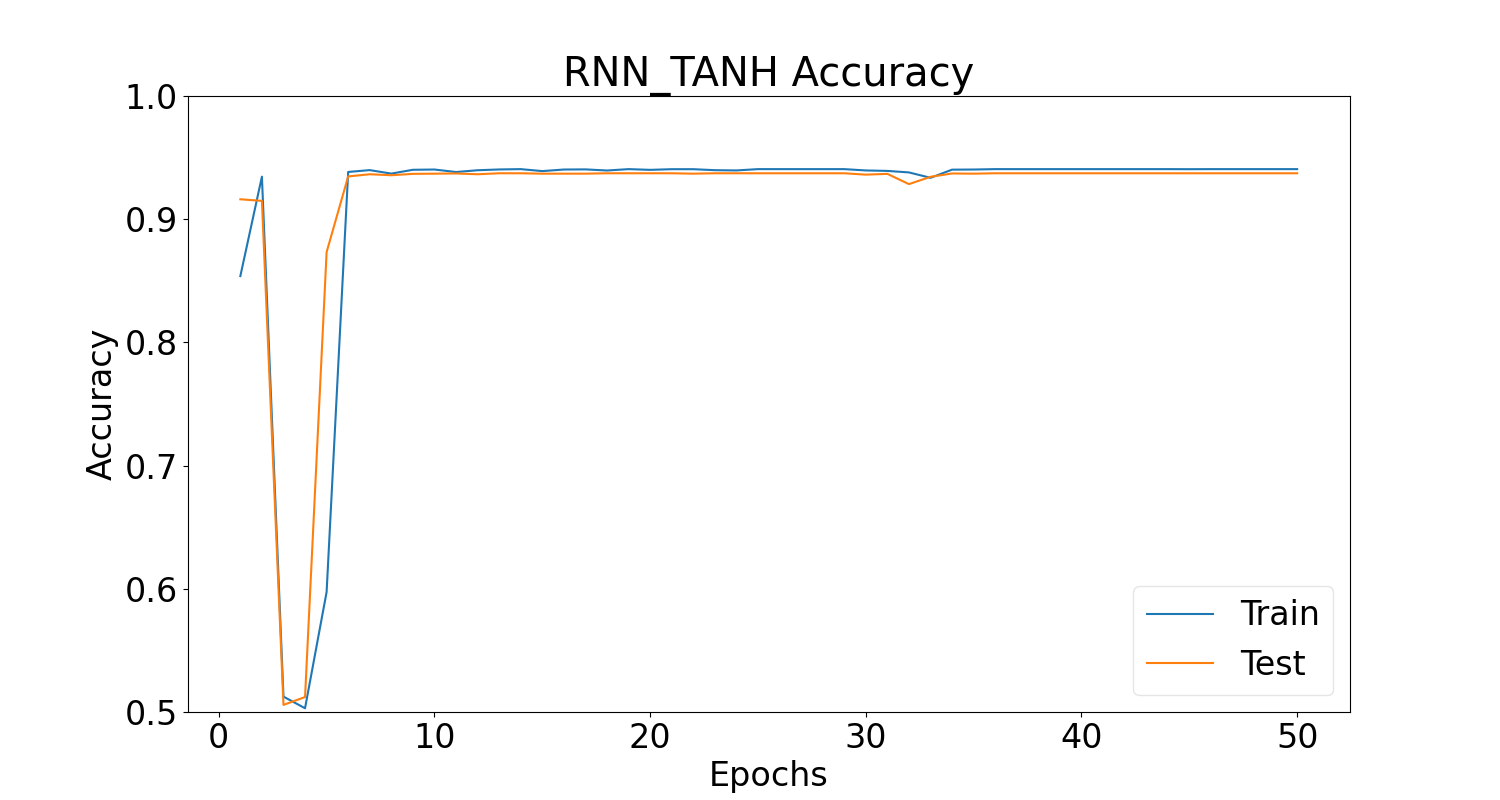
\includegraphics[width=0.82\linewidth]{images/results/base_model/rnn_tanh_accuracy.png}
	\caption[RNN\_Tanh base model performance]%
	{Base model performance of RNN with Tanh nonlinearity. This model is trained for 50 epochs with hyper-parameters shown in table \ref{tab:hype_param_base}.}
	\label{fig:rnn_tanh_bm}
\end{figure}

Next is the base model performance of RNN with ReLU nonlinearity. As we can see in the following graph, our model is consistently above $96\%$ accuracy throughout most of the training and evaluation phase.

\begin{figure}[h]
	\centering
	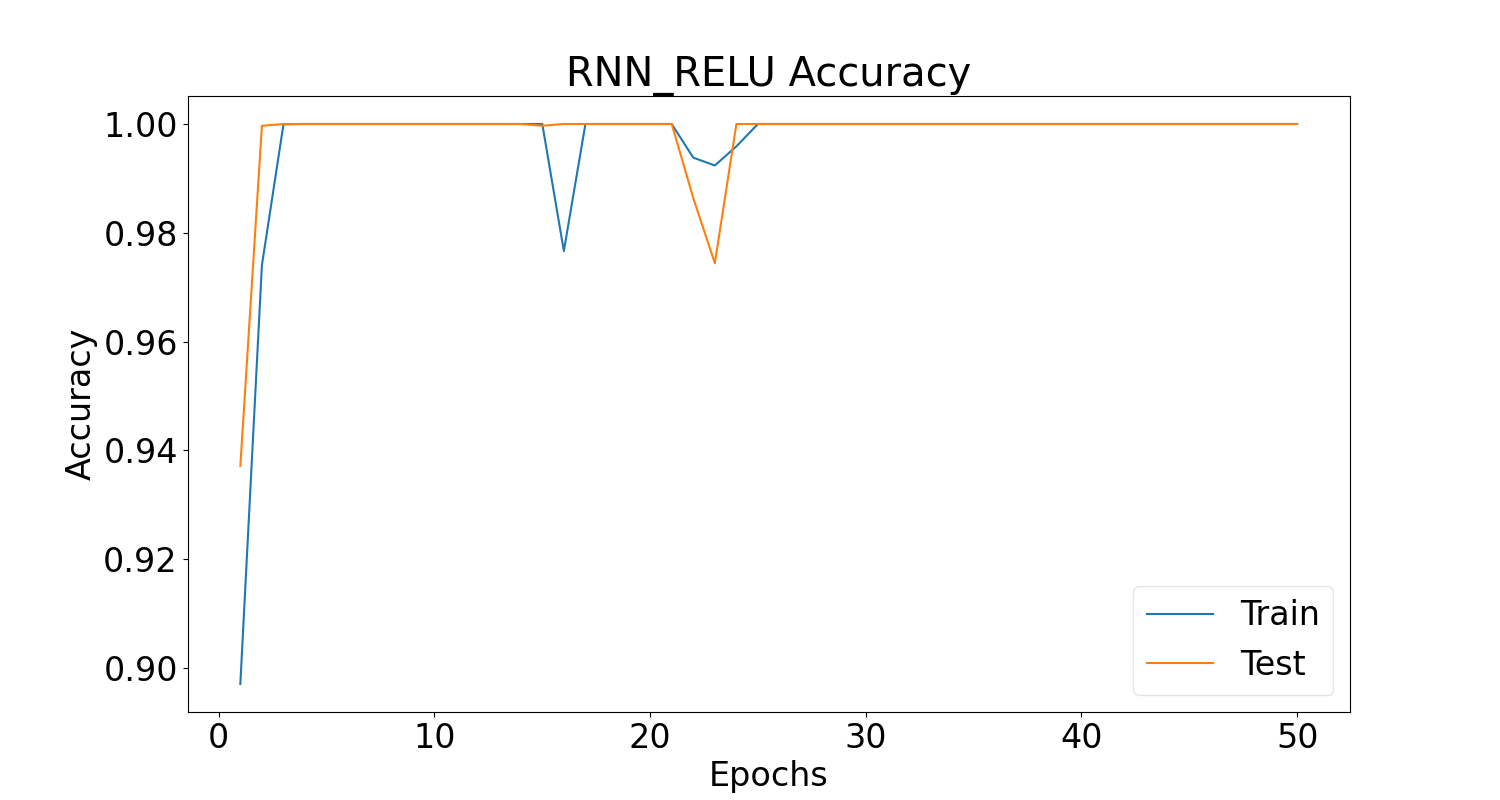
\includegraphics[width=0.82\linewidth]{images/results/base_model/rnn_relu_accuracy.png}
	\caption[RNN\_ReLU base model performance]%
	{Base model performance of RNN with ReLU nonlinearity. This model is trained for 50 epochs with hyper-parameters shown in table \ref{tab:hype_param_base}.}
	\label{fig:rnn_relu_bm}
\end{figure}

Our base LSTM model's performance is consistent at $100\%$ after beginning at around $93\%$ in the first epoch, as shown in the following figure:

\begin{figure}[h]
	\centering
	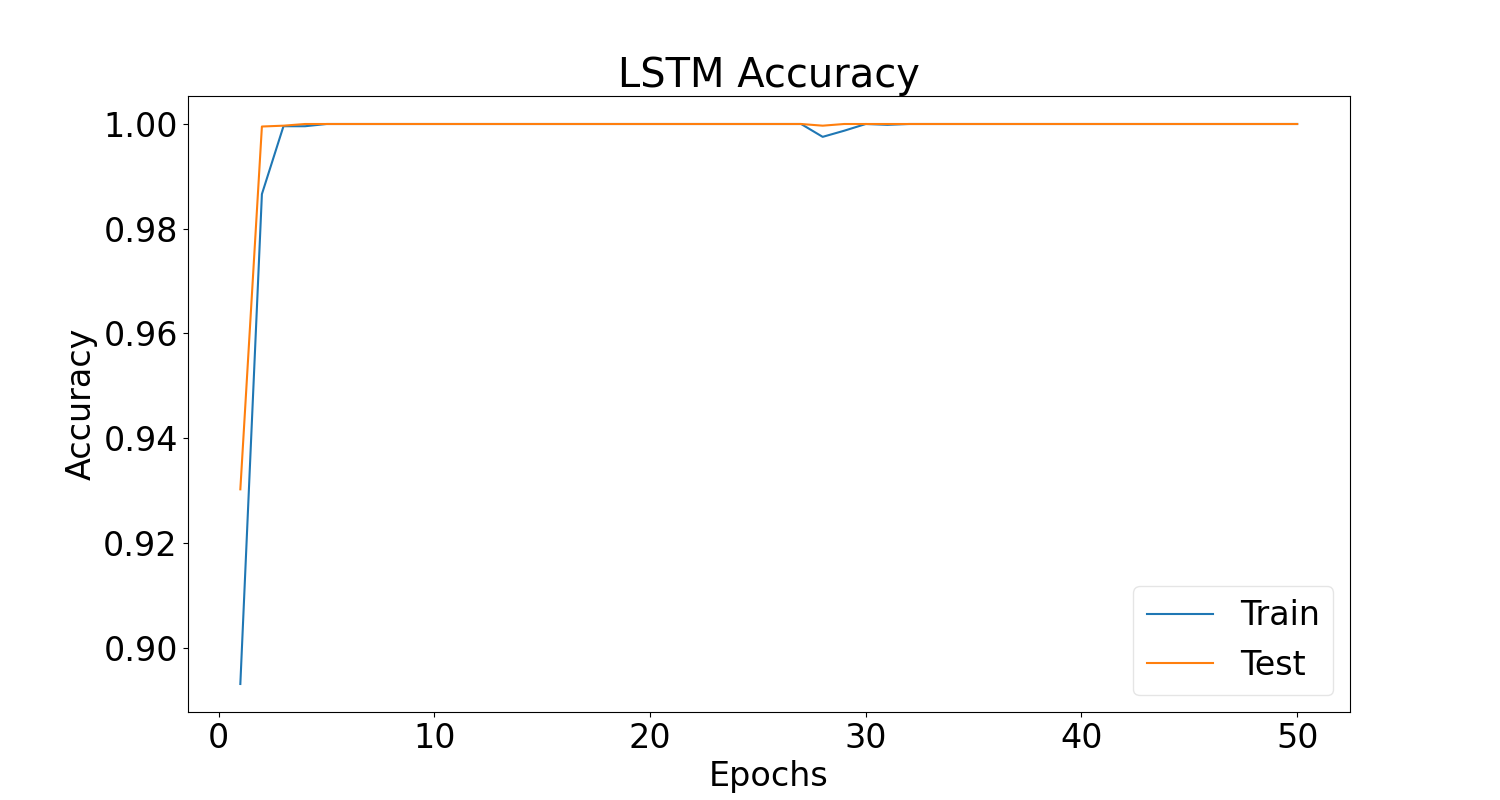
\includegraphics[width=0.82\linewidth]{images/results/base_model/lstm_accuracy.png}
	\caption[LSTM base model performance]%
	{Base model performance of LSTM. This model is trained for 50 epochs with hyper-parameters shown in table \ref{tab:hype_param_base}.}
	\label{fig:lstm_bm}
\end{figure}

Similar to LSTM, our base GRU model also performs consistently at $100\%$ after beginning at around $93\%$ in the first epoch, as shown in the following figure:

\begin{figure}[h]
	\centering
	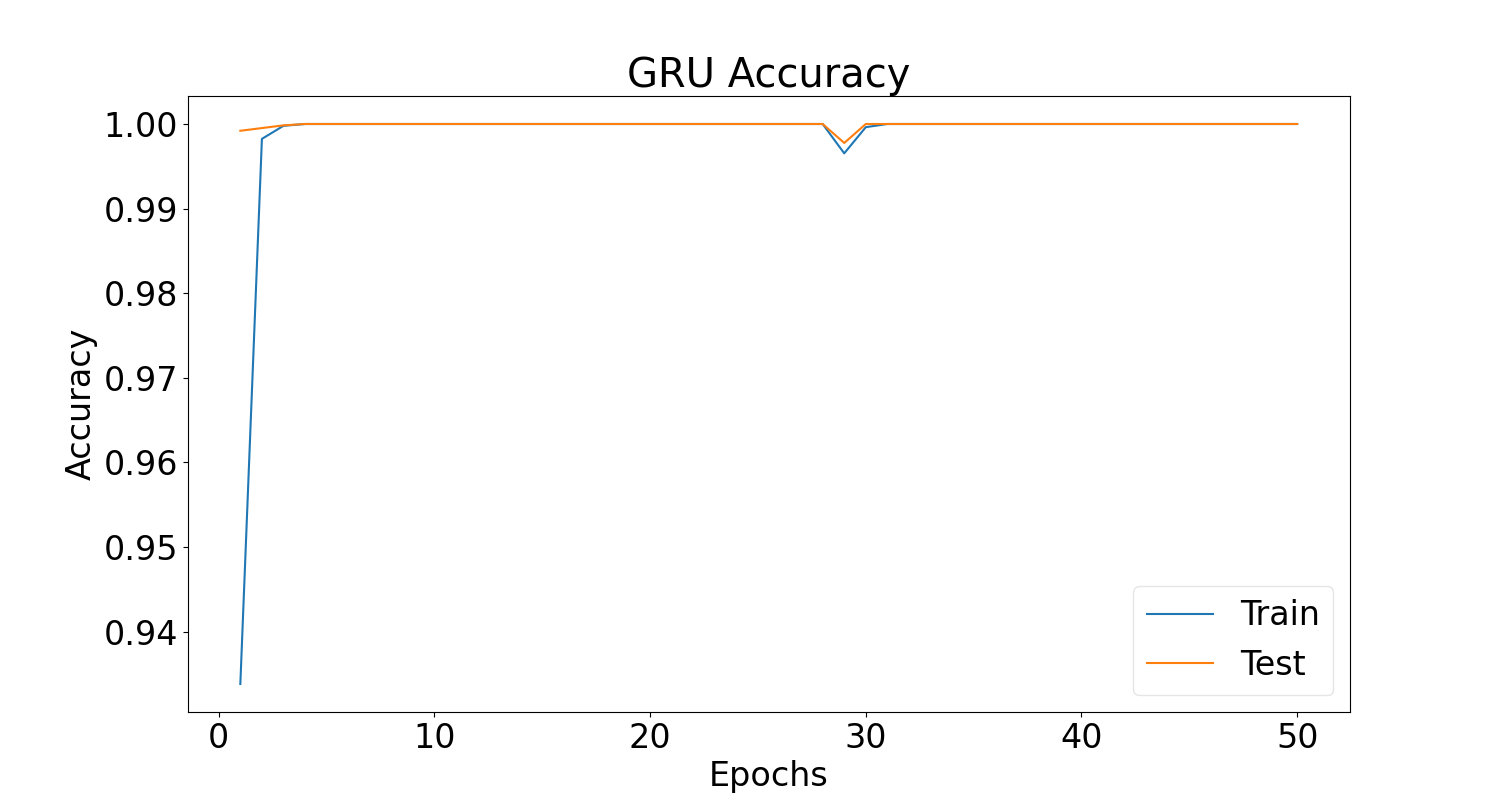
\includegraphics[width=0.82\linewidth]{images/results/base_model/gru_accuracy.png}
	\caption[GRU base model performance]%
	{Base model performance of GRU. This model is trained for 50 epochs with hyper-parameters shown in table \ref{tab:hype_param_base}.}
	\label{fig:gru_bm}
\end{figure}

Next, we look at the performance of our base model after pruning it.

% -----------------------------------------------------------------------------------------------------------
% ------------------------------------------------- PRUNING -------------------------------------------------
% -----------------------------------------------------------------------------------------------------------

\section{Base model performance after pruning}

We begin with displaying the results of pruning both input-to-hidden and hidden-to-hidden weights for each RNN variant, then we proceed with the results of pruning only input-to-hidden weights, and later, the results of pruning only hidden-to-hidden weights.

In each section, we also present the visualizations showing the number of epochs required to regain accuracy after pruning each RNN variant's models.

\subsection[Pruning both, input-to-hidden and hidden-to-hidden weights]{Pruning input-to-hidden and hidden-to-hidden weights simultaneously}

First, we look at performance of RNN with Tanh nonlinearity after applying $10\%$ to $100\%$ pruning. As we can see in figure \ref{fig:rnn_tanh_prune}, the model performs consistently at above 90\% accuracy at 80\% pruning, meaning the model retains near original performance with 80\% fewer parameters. The model observes a sharp decline in performance at 90\% pruning and goes to baseline accuracy at 100\% pruning.

\begin{figure}[h]
	\centering
	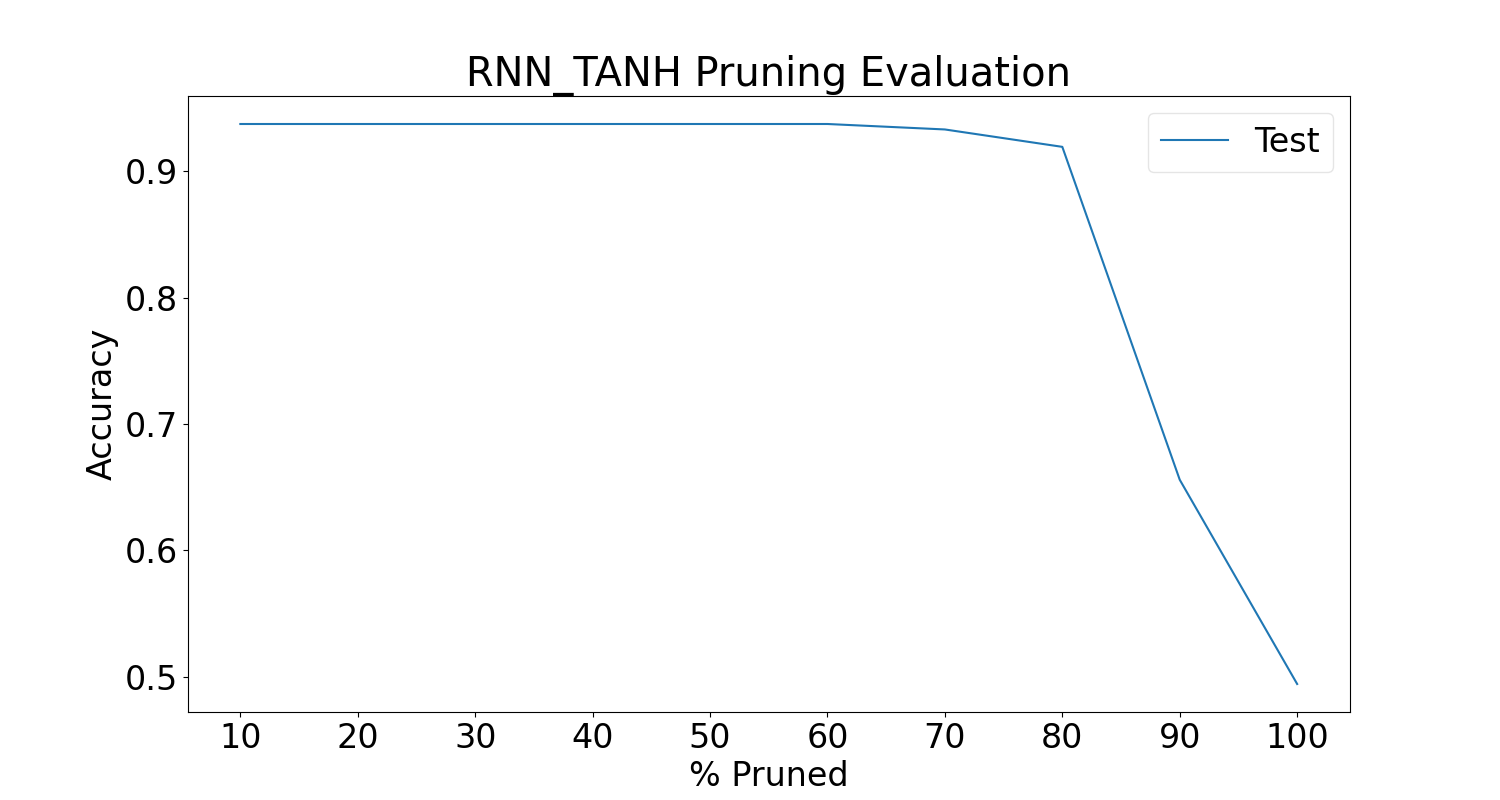
\includegraphics[width=0.8\linewidth]{images/results/pruning/rnn_tanh_pruning_evaluation.png}
	\caption[RNN\_Tanh base model performance after pruning]%
	{Base model performance of RNN\_Tanh after pruning. The pruning starts from $10\%$ and ends at $100\%$ with an increment of $10$ after each pruning round.}
	\label{fig:rnn_tanh_prune}
\end{figure}

Next, we observe the number of epochs the model requires to regain the accuracy at 80\%, 90\%, and 100\% pruning:

\begin{figure}[h]
	\centering
	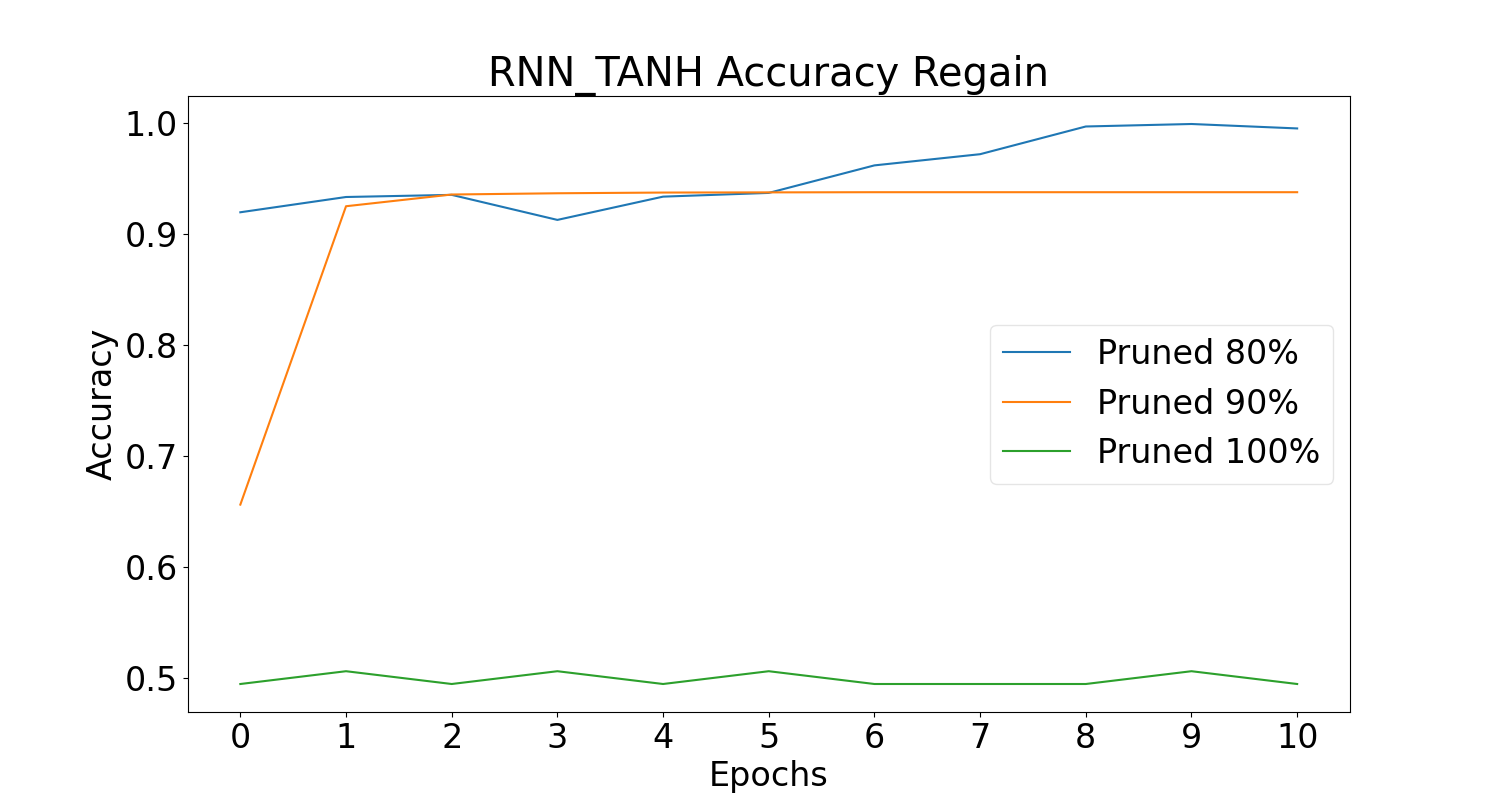
\includegraphics[width=0.8\linewidth]{images/results/pruning/rnn_tanh_accuracy_regain.png}
	\caption[RNN\_Tanh base model performance regain after pruning]%
	{The number of epochs required to regain the accuracy of RNN\_Tanh model after applying 80\%, 90\%, and 100\% pruning.}
	\label{fig:rnn_tanh_prune_regain}
\end{figure}

As we can see in the above figure, after pruning 80\% and 90\% of input-to-hidden and hidden-to-hidden weights, the model regains the original above 90\% performance only after one epoch, while the model never recovers at 100\% pruning.

Next, we look at performance of RNN with ReLU nonlinearity after applying $10\%$ to $100\%$ pruning. As we can see in figure \ref{fig:rnn_relu_prune}, the model performs consistently at above 90\% accuracy at 70\% pruning, meaning the model retains near original performance with 70\% fewer parameters. The model observes a sharp decline in performance at 80\% pruning and goes to baseline accuracy at 100\% pruning.

\begin{figure}[h]
	\centering
	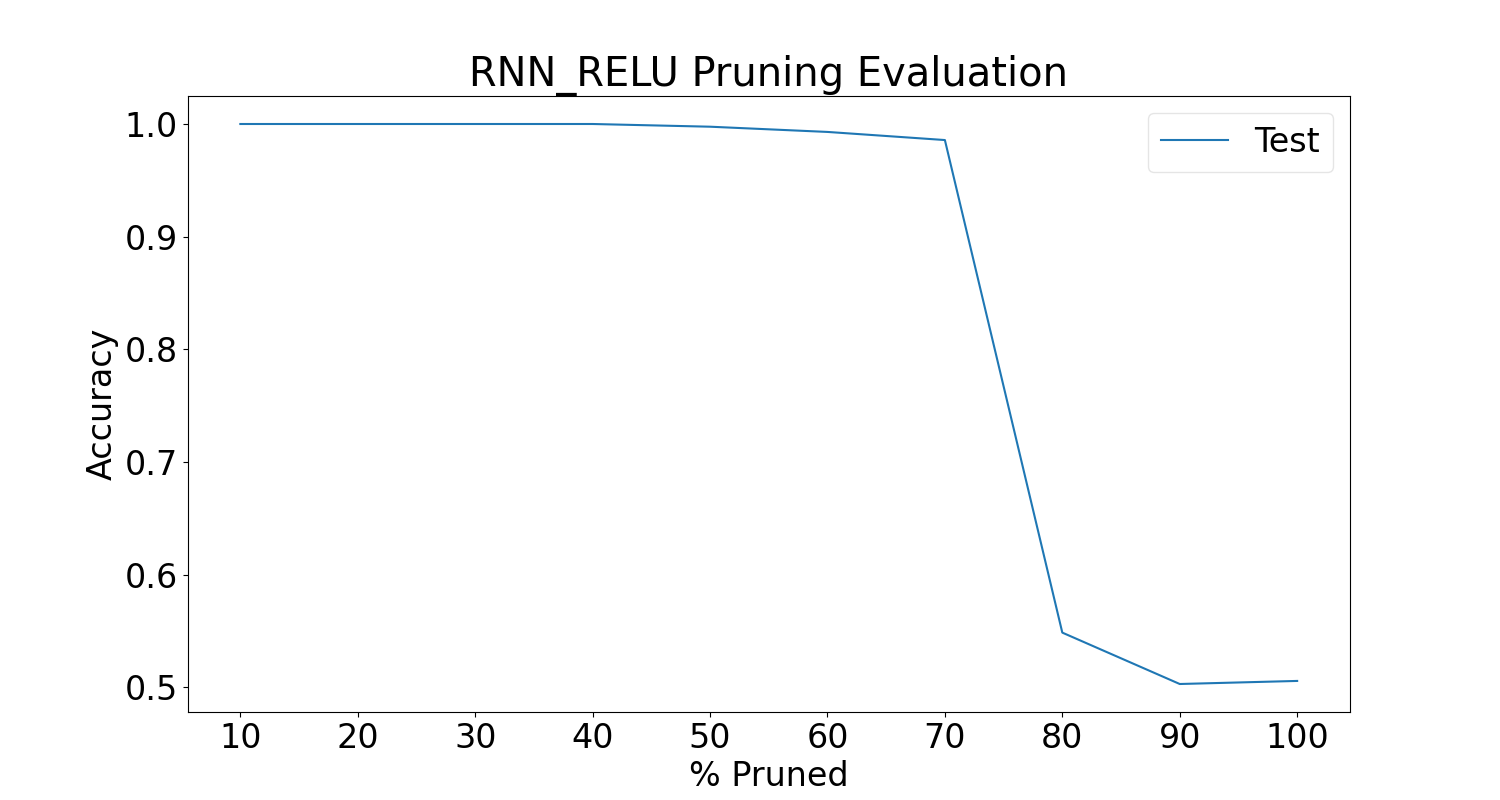
\includegraphics[width=0.8\linewidth]{images/results/pruning/rnn_relu_pruning_evaluation.png}
	\caption[RNN\_ReLU base model performance after pruning]%
	{Base model performance of RNN\_ReLU after pruning. The pruning starts from $10\%$ and ends at $100\%$ with an increment of $10$ after each pruning round.}
	\label{fig:rnn_relu_prune}
\end{figure}

Next, we observe the number of epochs the model requires to regain the accuracy at 80\%, 90\%, and 100\% pruning:

\begin{figure}[h]
	\centering
	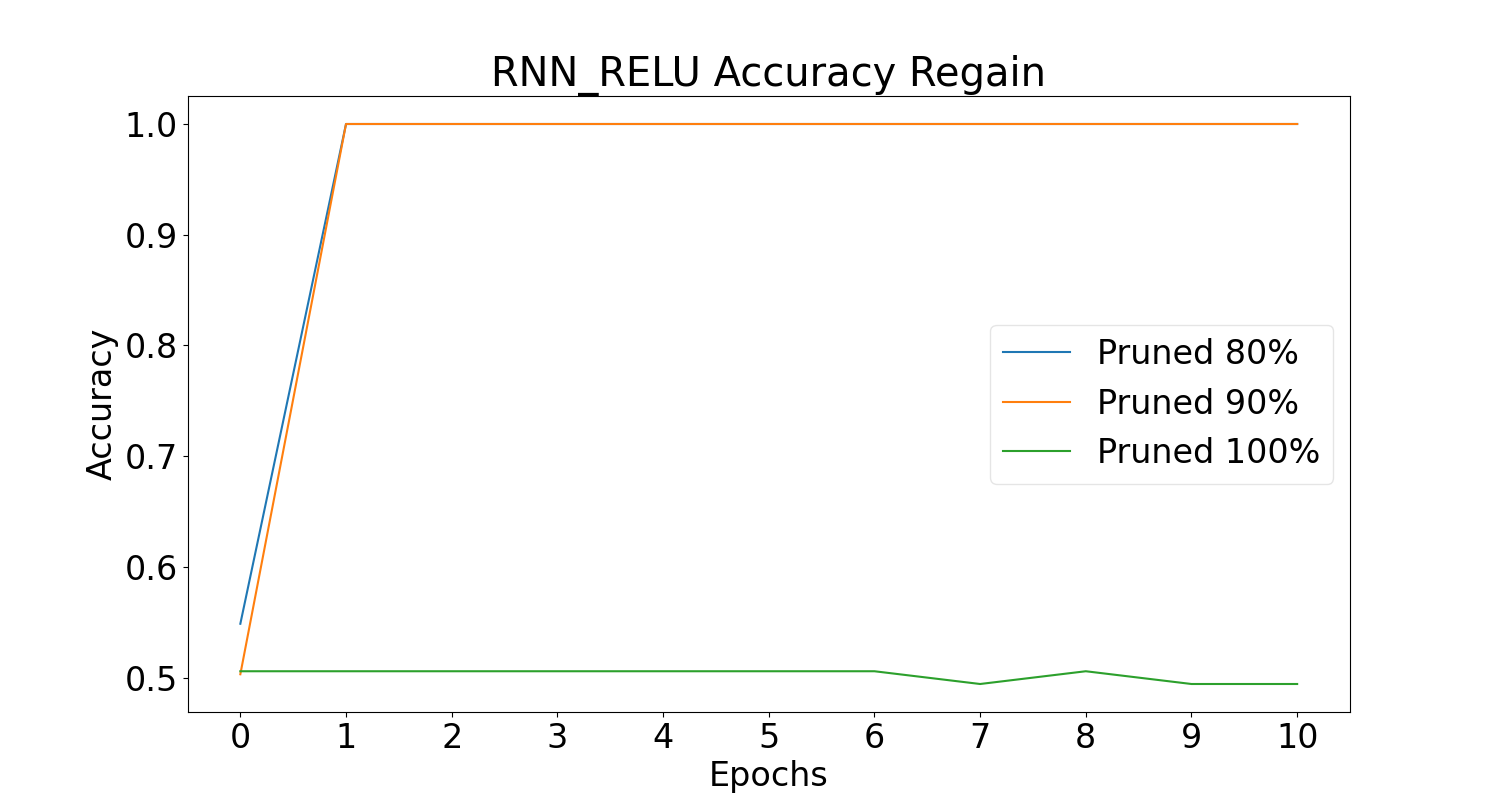
\includegraphics[width=0.8\linewidth]{images/results/pruning/rnn_relu_accuracy_regain.png}
	\caption[RNN\_ReLU base model performance regain after pruning]%
	{The number of epochs required to regain the accuracy of RNN\_ReLU model after applying 80\%, 90\%, and 100\% pruning.}
	\label{fig:rnn_relu_prune_regain}
\end{figure}

Similar to RNN\_Tanh, after pruning 80\% and 90\% of input-to-hidden and hidden-to-hidden weights, the model regains the original 100\% accuracy only after one epoch, while the model never recovers at 100\% pruning.

Next, we look at performance of LSTM model after applying $10\%$ to $100\%$ pruning. As we can see in figure \ref{fig:lstm_prune}, the model performs consistently at 100\% accuracy at 60\% pruning. The model observes a sharp decline in performance at 70\% pruning and goes to baseline accuracy at 90\% pruning.

\begin{figure}[h]
	\centering
	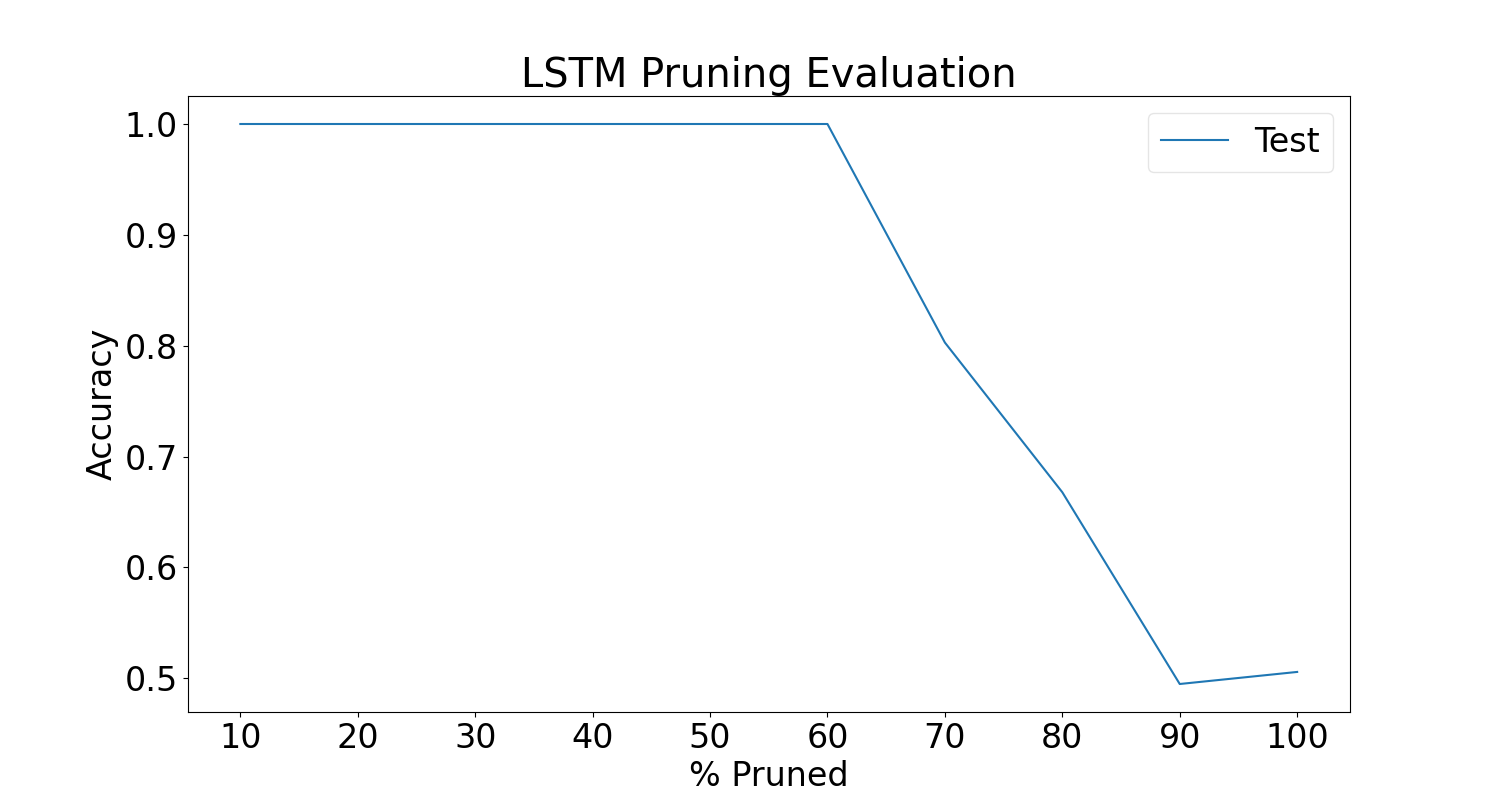
\includegraphics[width=0.8\linewidth]{images/results/pruning/lstm_pruning_evaluation.png}
	\caption[LSTM base model performance after pruning]%
	{Base model performance of LSTM model after pruning. The pruning starts from $10\%$ and ends at $100\%$ with an increment of $10$ after each pruning round.}
	\label{fig:lstm_prune}
\end{figure}

Next, we observe the number of epochs the model requires to regain the accuracy at 70\%, 80\%, 90\%, and 100\% pruning:

\begin{figure}[h]
	\centering
	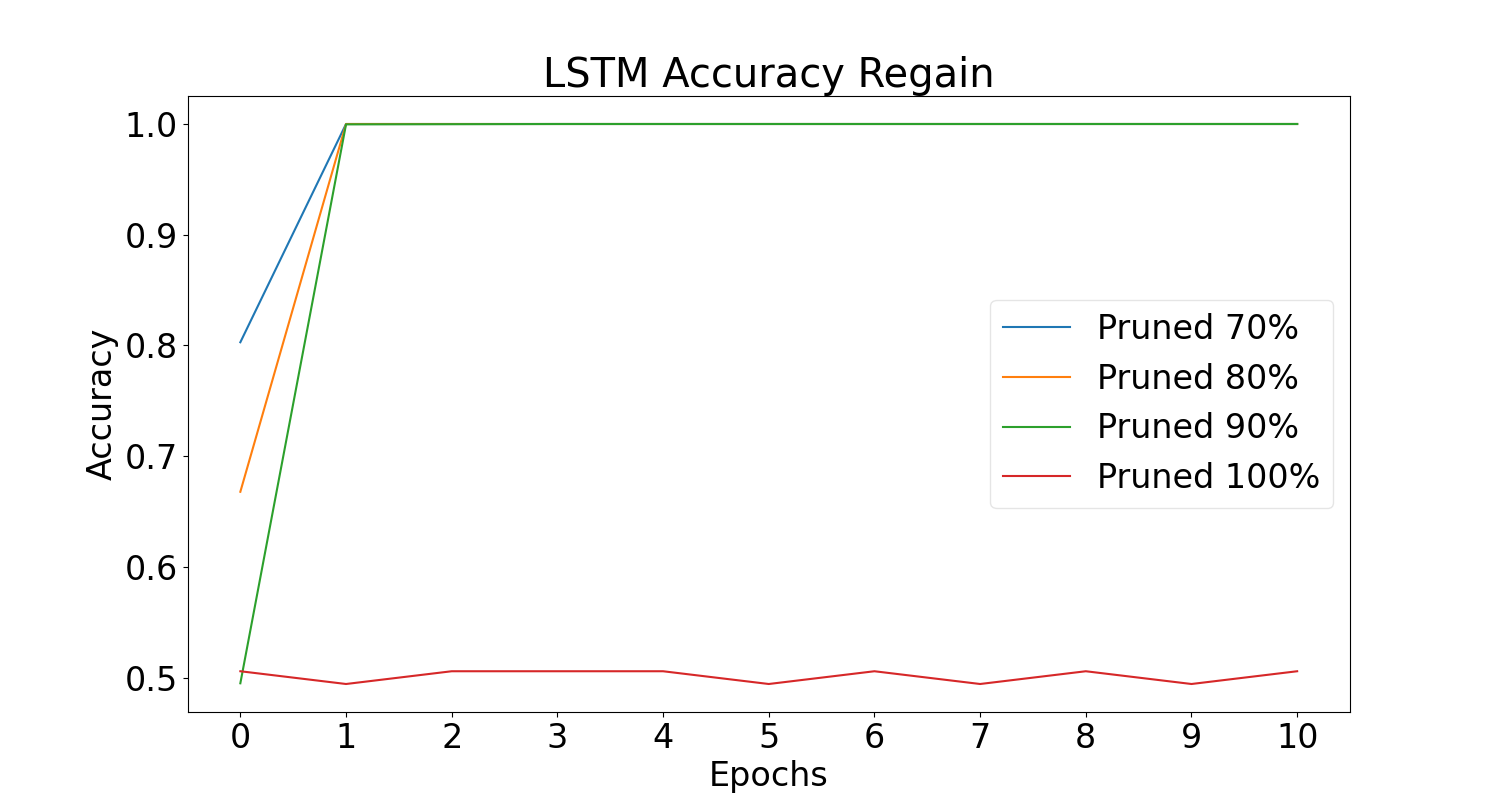
\includegraphics[width=0.8\linewidth]{images/results/pruning/lstm_accuracy_regain.png}
	\caption[LSTM base model performance regain after pruning]%
	{The number of epochs required to regain the accuracy of LSTM model after applying 70\%, 80\%, 90\%, and 100\% pruning.}
	\label{fig:lstm_prune_regain}
\end{figure}

Similar to RNN\_Tanh and RNN\_ReLU, after pruning 70\%, 80\% and 90\% of input-to-hidden and hidden-to-hidden weights, the model regains the original 100\% accuracy only after one epoch, while the model never recovers at 100\% pruning.

Finally, we look at performance of GRU model after applying $10\%$ to $100\%$ pruning. As we can see in figure \ref{fig:gru_prune}, the model performs consistently at near 100\% accuracy at 80\% pruning. The model observes a sharp decline in performance at 90\% pruning and goes to baseline accuracy at 100\% pruning.

\begin{figure}[h]
	\centering
	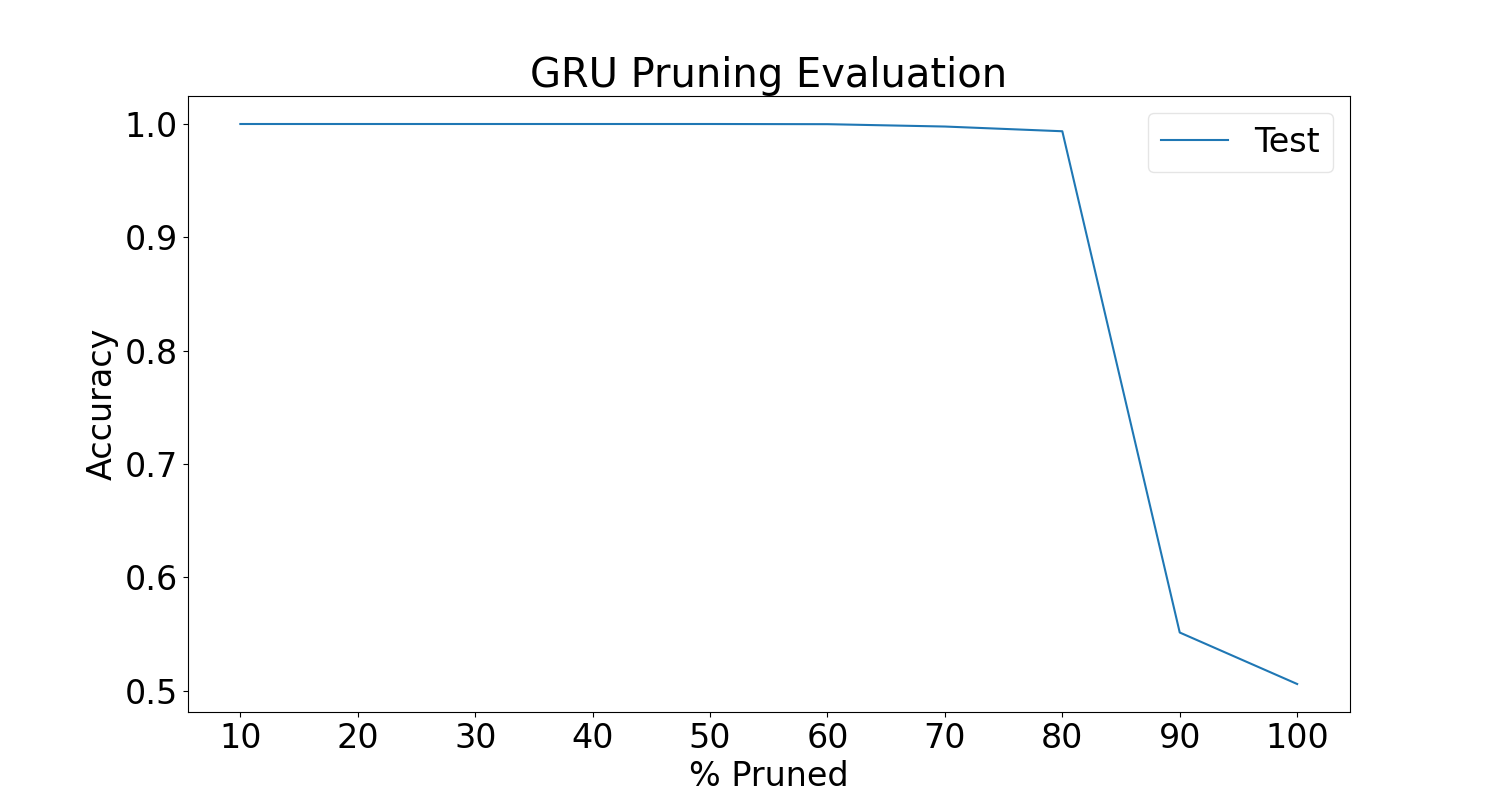
\includegraphics[width=0.8\linewidth]{images/results/pruning/gru_pruning_evaluation.png}
	\caption[GRU base model performance after pruning]%
	{Base model performance of GRU model after pruning. The pruning starts from $10\%$ and ends at $100\%$ with an increment of $10$ after each pruning round.}
	\label{fig:gru_prune}
\end{figure}

Next, we observe the number of epochs the model requires to regain the accuracy at 90\%, and 100\% pruning:

\begin{figure}[h]
	\centering
	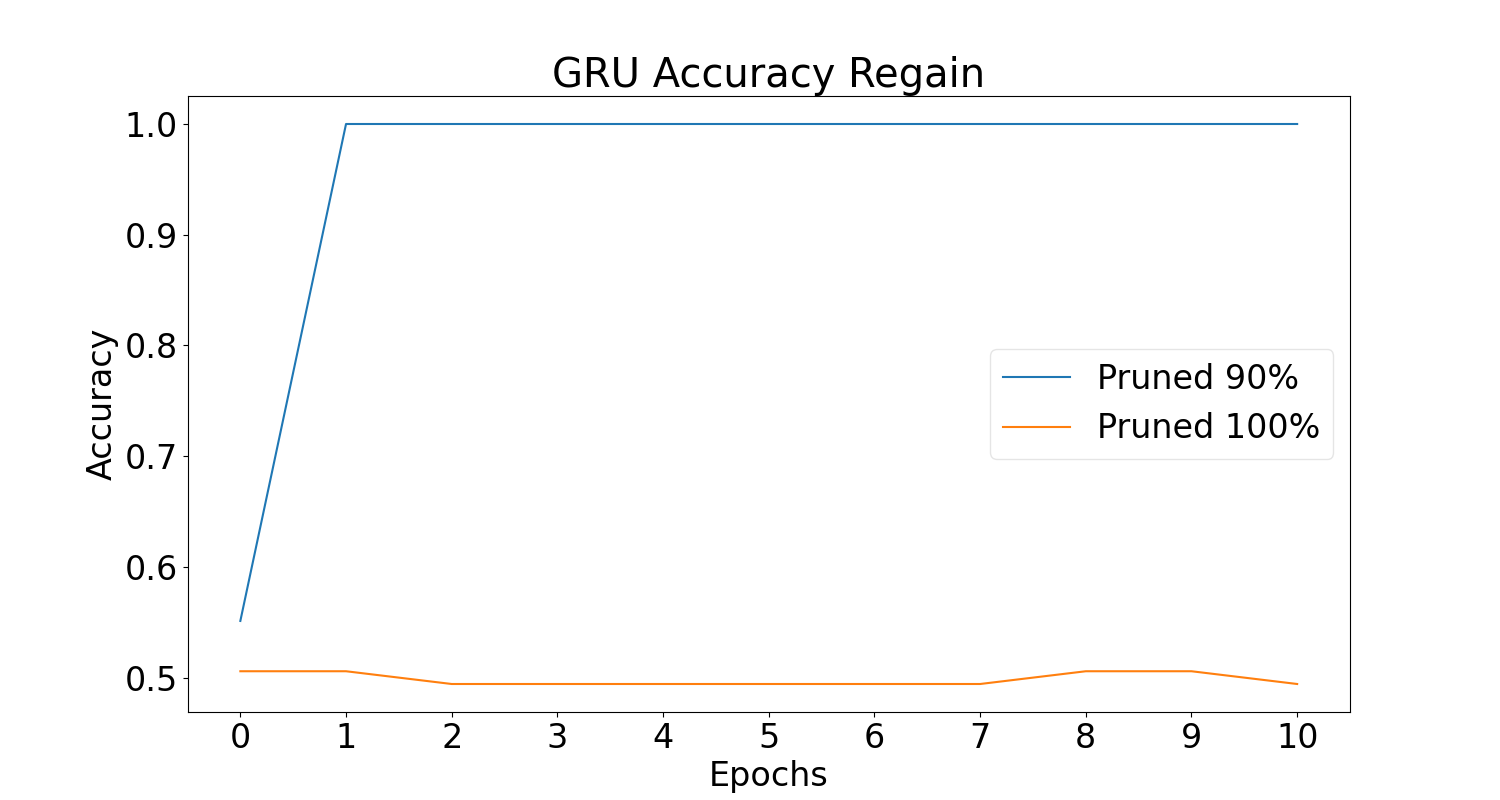
\includegraphics[width=0.8\linewidth]{images/results/pruning/gru_accuracy_regain.png}
	\caption[GRU base model performance regain after pruning]%
	{The number of epochs required to regain the accuracy of GRU model after applying 90\%, and 100\% pruning.}
	\label{fig:gru_prune_regain}
\end{figure}

Similar to RNN\_Tanh, RNN\_ReLU, and LSTM, after pruning 90\% of input-to-hidden and hidden-to-hidden weights, the model regains the original 100\% accuracy only after one epoch, while the model never recovers at 100\% pruning.

\subsection{Pruning only input-to-hidden weights}

In this section, we present the results of pruning only input-to-hidden weights in our base model.

First, we look at how pruning only input-to-hidden weights affect the performance of RNN with Tanh nonlinearity. As shown in figure \ref{fig:rnn_tanh_i2h_prune}, the model performs consistently at above 90\% accuracy with 70\% of input-to-hidden weights pruned. We observe a sharp drop in accuracy at 80\% pruning.

\begin{figure}[h]
	\centering
	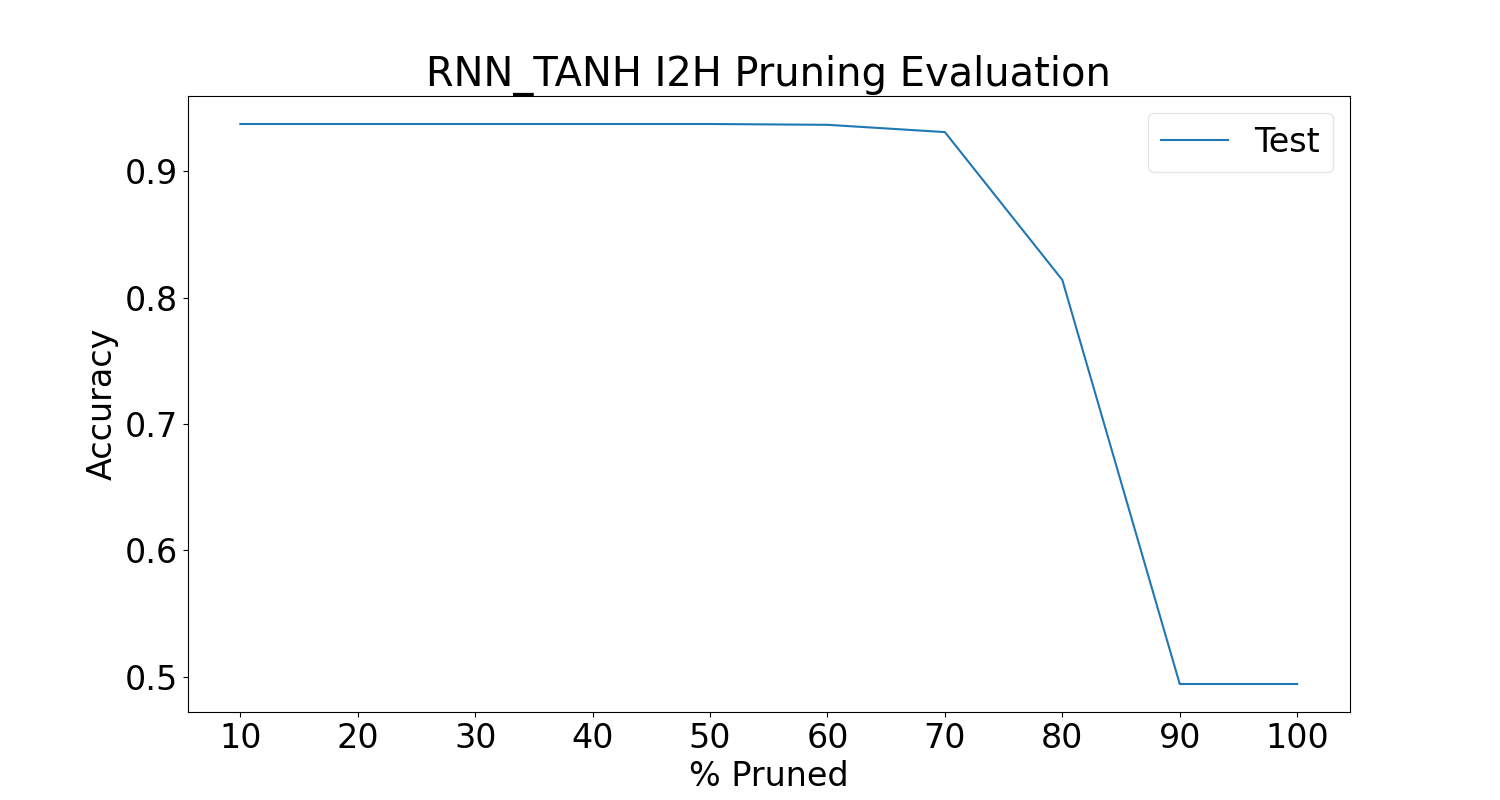
\includegraphics[width=0.8\linewidth]{images/results/pruning_i2h/rnn_tanh_i2h_pruning_evaluation.png}
	\caption[RNN\_Tanh base model performance after pruning i2h weights]%
	{Base model performance of RNN with Tanh nonlinearity after pruning only input-to-hidden weights. The pruning starts from $10\%$ and ends at $100\%$ with an increment of $10$ after each pruning round.}
	\label{fig:rnn_tanh_i2h_prune}
\end{figure}

As shown in the above figure, the model starts performing worse from 80\% pruning and above. Figure \ref{fig:rnn_tanh_i2h_prune_regain} shows the number of epochs it takes for this pruned model to regain accuracy after pruning 80\%, 90\%, and 100\% of input-to-hidden weights.

As shown, the model regains above 90\% accuracy only after one epoch with 80\% pruning, while it takes two epochs to regain accuracy after 90\% pruning. The model never recovers after pruning 100\% of input-to-hidden weights.

\begin{figure}[h]
	\centering
	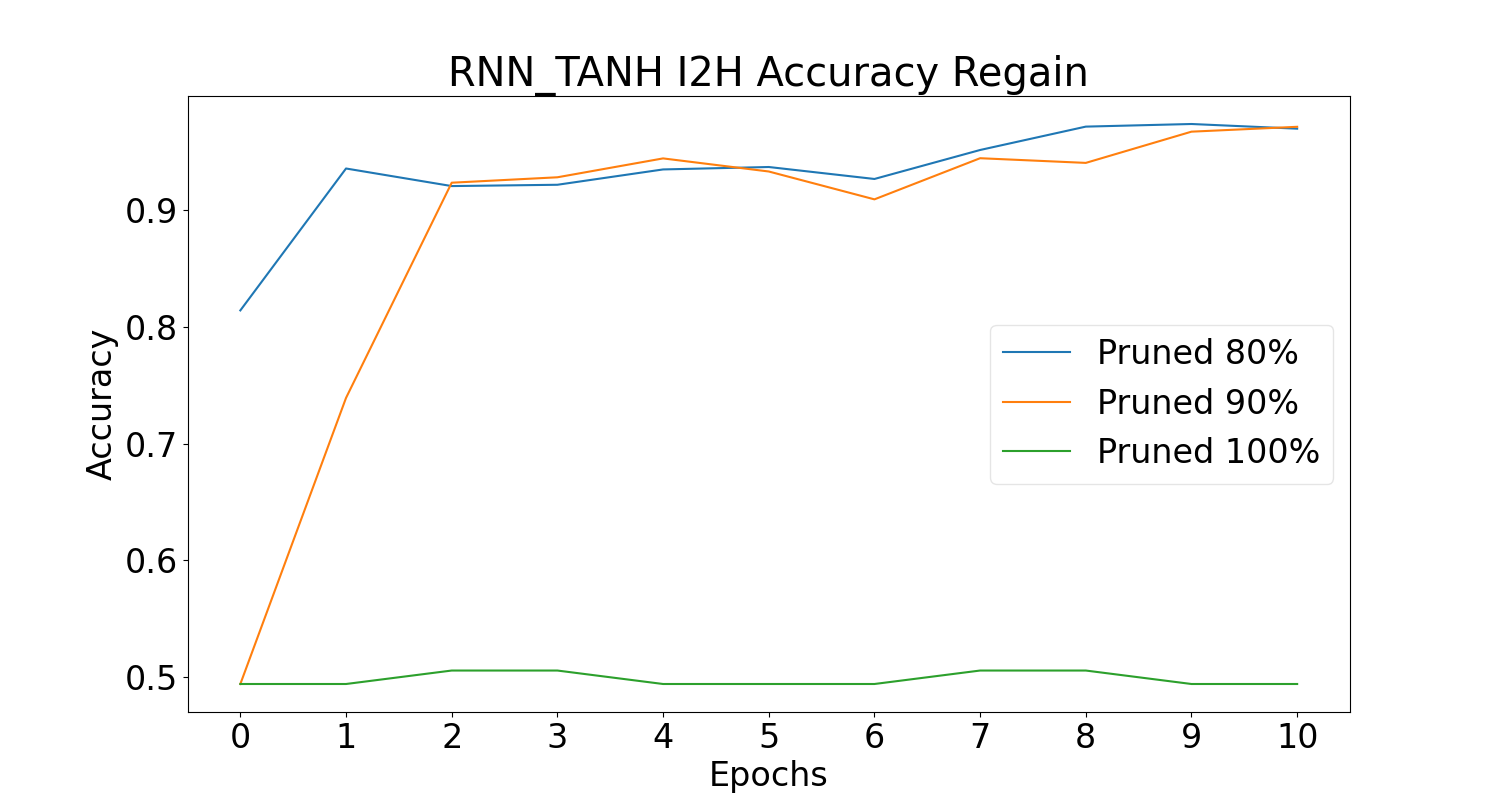
\includegraphics[width=0.8\linewidth]{images/results/pruning_i2h/rnn_tanh_i2h_accuracy_regain.png}
	\caption[RNN\_Tanh base model performance regain after pruning i2h weights]%
	{The number of epochs required to regain the accuracy of RNN\_Tanh model after pruning 80\%, 90\%, and 100\% of input-to-hidden weights.}
	\label{fig:rnn_tanh_i2h_prune_regain}
\end{figure}

Next, we look at how pruning only input-to-hidden weights affect the performance of RNN with ReLU nonlinearity. As shown in figure \ref{fig:rnn_relu_i2h_prune}, the model performs consistently at above 90\% accuracy with 80\% of input-to-hidden weights pruned. We observe a sharp drop in accuracy at 90\% pruning.

\begin{figure}[H]
	\centering
	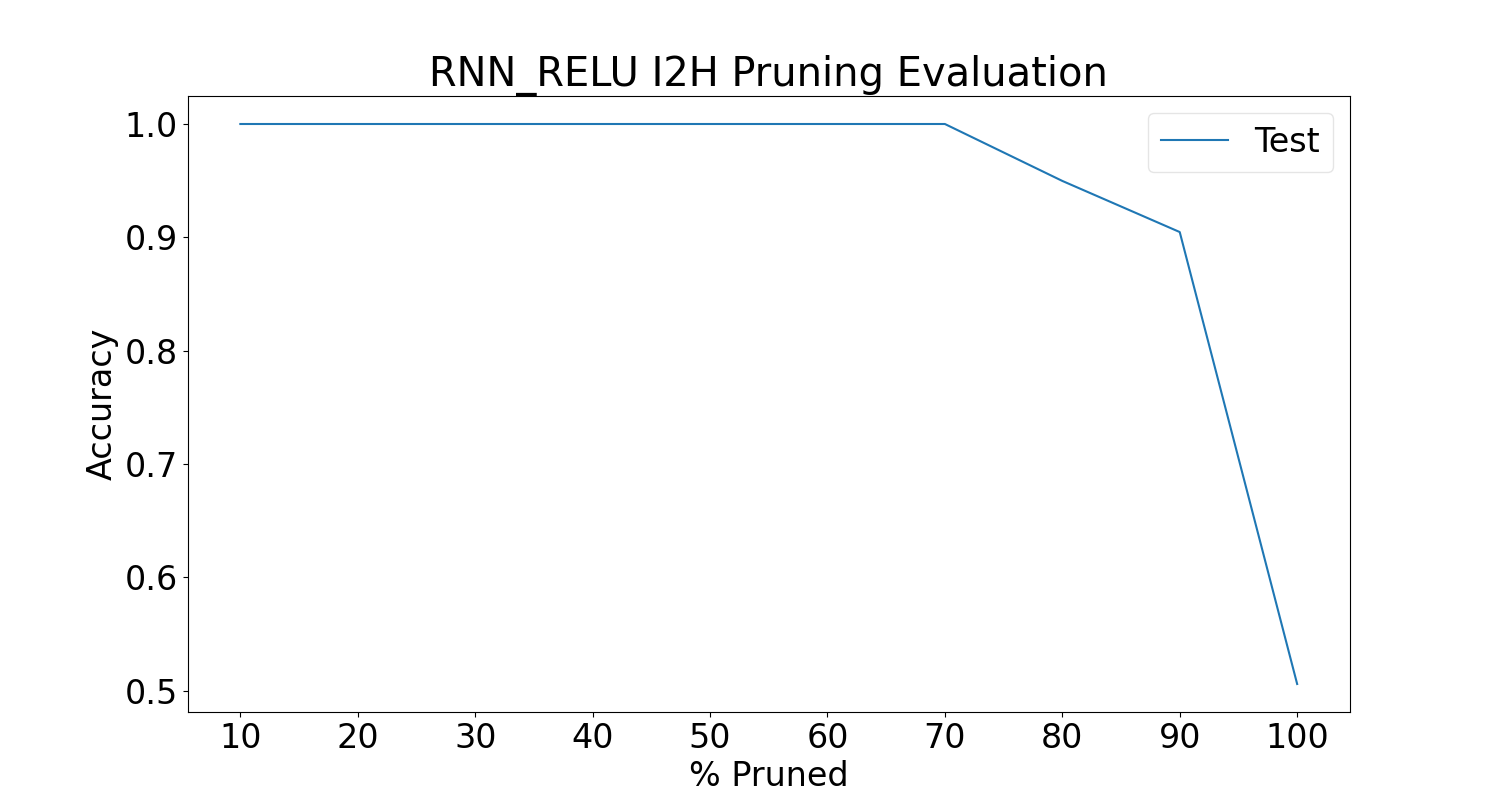
\includegraphics[width=0.8\linewidth]{images/results/pruning_i2h/rnn_relu_i2h_pruning_evaluation.png}
	\caption[RNN\_ReLU base model performance after pruning i2h weights]%
	{Base model performance of RNN with ReLU nonlinearity after pruning only input-to-hidden weights. The pruning starts from $10\%$ and ends at $100\%$ with an increment of $10$ after each pruning round.}
	\label{fig:rnn_relu_i2h_prune}
\end{figure}

As shown in the above figure, the model starts dropping accuracy from 80\% pruning and above. Figure \ref{fig:rnn_relu_i2h_prune_regain} shows the number of epochs it takes for this pruned model to regain accuracy after pruning 80\%, 90\%, and 100\% of input-to-hidden weights.

\begin{figure}[h]
	\centering
	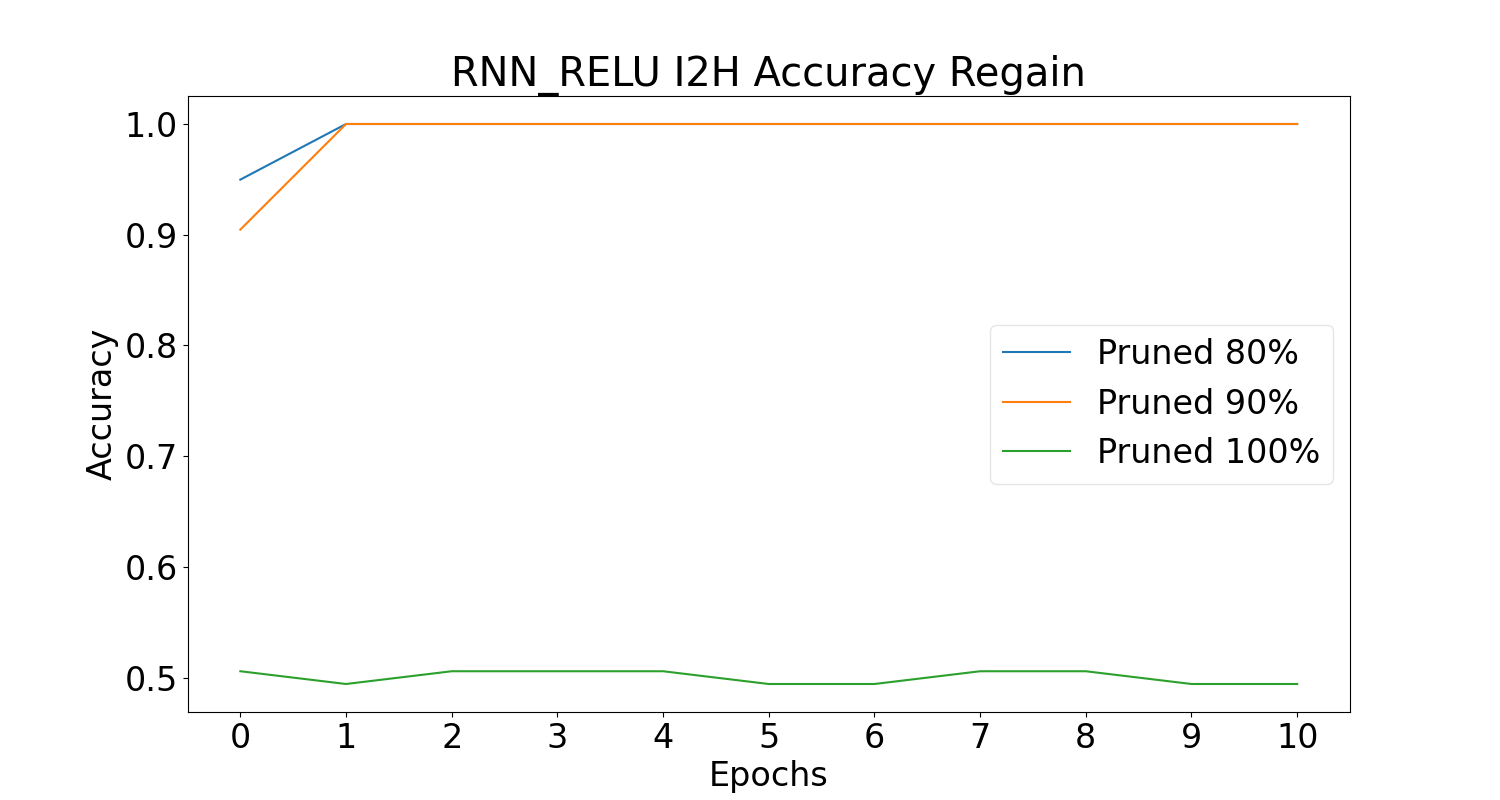
\includegraphics[width=0.8\linewidth]{images/results/pruning_i2h/rnn_relu_i2h_accuracy_regain.png}
	\caption[RNN\_ReLU base model performance regain after pruning i2h weights]%
	{The number of epochs required to regain the accuracy of RNN\_ReLU model after pruning 80\%, 90\%, and 100\% of input-to-hidden weights.}
	\label{fig:rnn_relu_i2h_prune_regain}
\end{figure}

As shown, the model regains above 90\% accuracy only after one epoch with 80\% and 90\% pruning, while the model never recovers after pruning 100\% of input-to-hidden weights.

Next, the following graph shows the effect of pruning only input-to-hidden weights on our LSTM model's performance:

\begin{figure}[h]
	\centering
	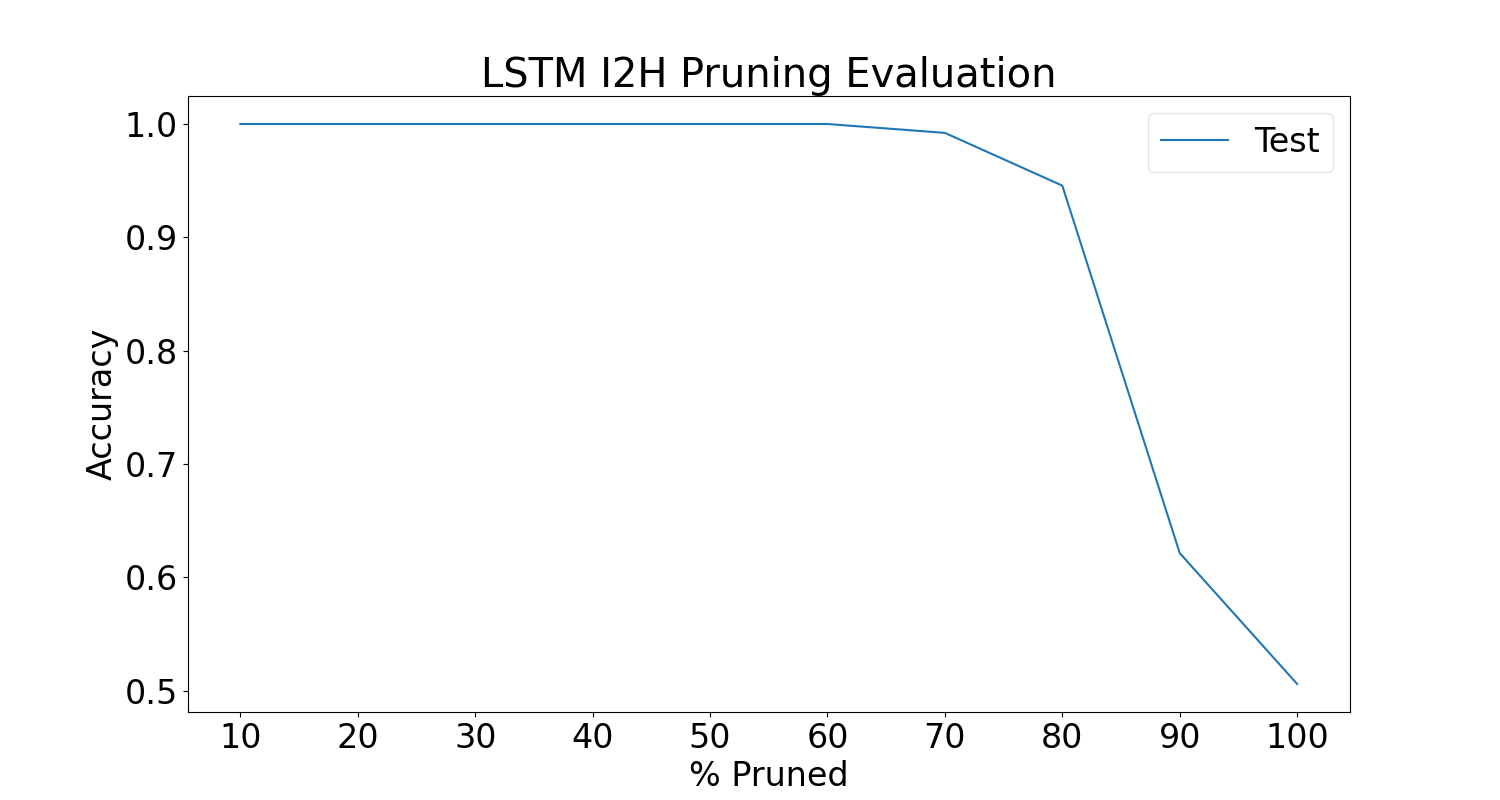
\includegraphics[width=0.8\linewidth]{images/results/pruning_i2h/lstm_i2h_pruning_evaluation.png}
	\caption[LSTM base model performance after pruning i2h weights]%
	{Base model performance of LSTM after pruning only input-to-hidden weights. The pruning starts from $10\%$ and ends at $100\%$ with an increment of $10$ after each pruning round.}
	\label{fig:lstm_i2h_prune}
\end{figure}

As we can see in the above graph, the model performs consistently at around 95\% accuracy with 80\% pruning. The model's performance drops sharply at 90\% pruning and returns baseline accuracy at 100\% pruning. Figure \ref{fig:lstm_i2h_prune_regain} shows the number of epochs it takes for the LSTM model to recover after pruning 80\%, 90\%, and 100\% of its input-to-hidden weights.

\begin{figure}[h]
	\centering
	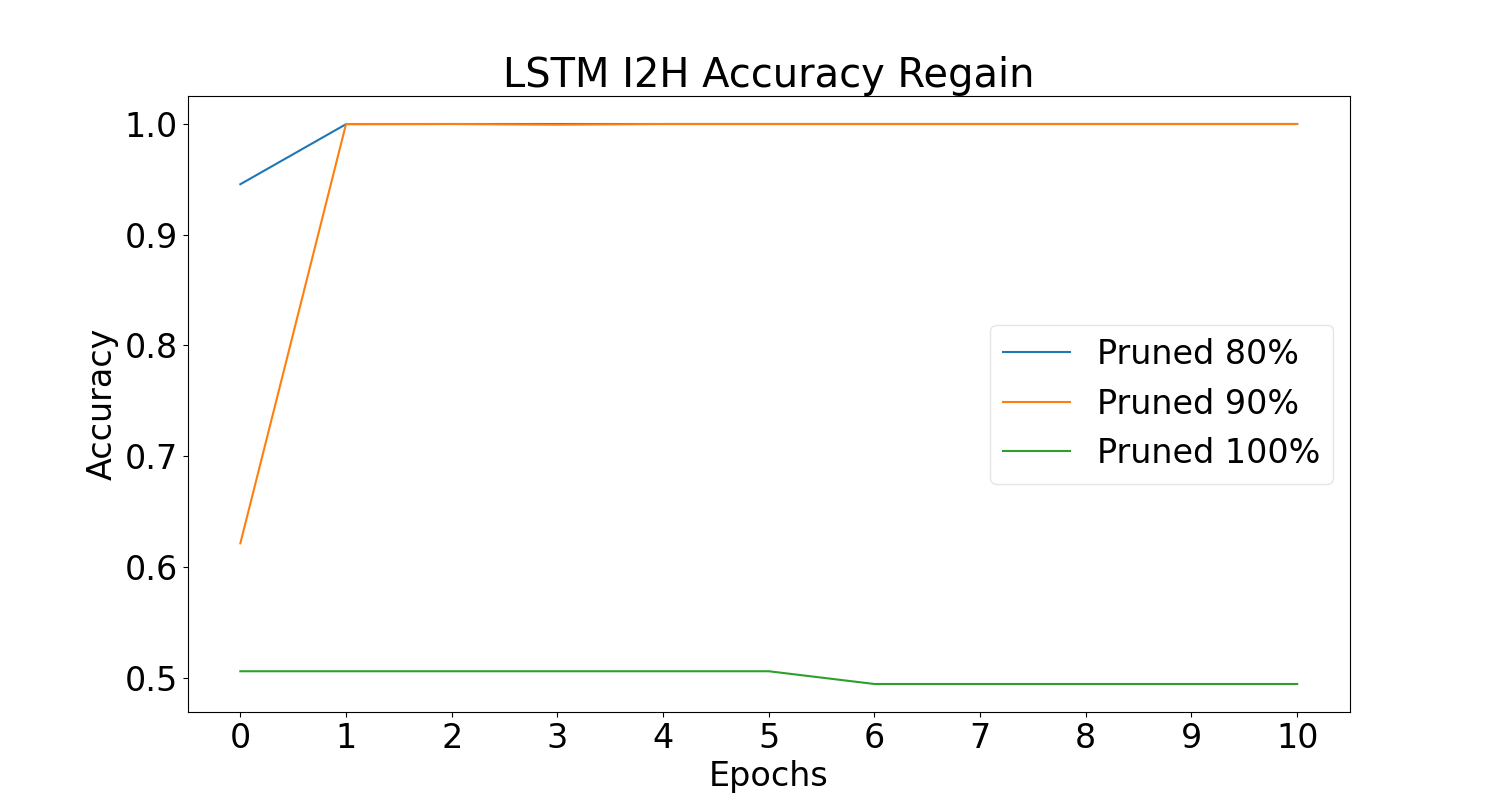
\includegraphics[width=0.8\linewidth]{images/results/pruning_i2h/lstm_i2h_accuracy_regain.png}
	\caption[LSTM base model performance regain after pruning i2h weights]%
	{The number of epochs required to regain the accuracy of LSTM model after pruning 80\%, 90\%, and 100\% of input-to-hidden weights.}
	\label{fig:lstm_i2h_prune_regain}
\end{figure}

Finally, the following graph shows the effect of pruning only input-to-hidden weights on our GRU model's performance:

\begin{figure}[h]
	\centering
	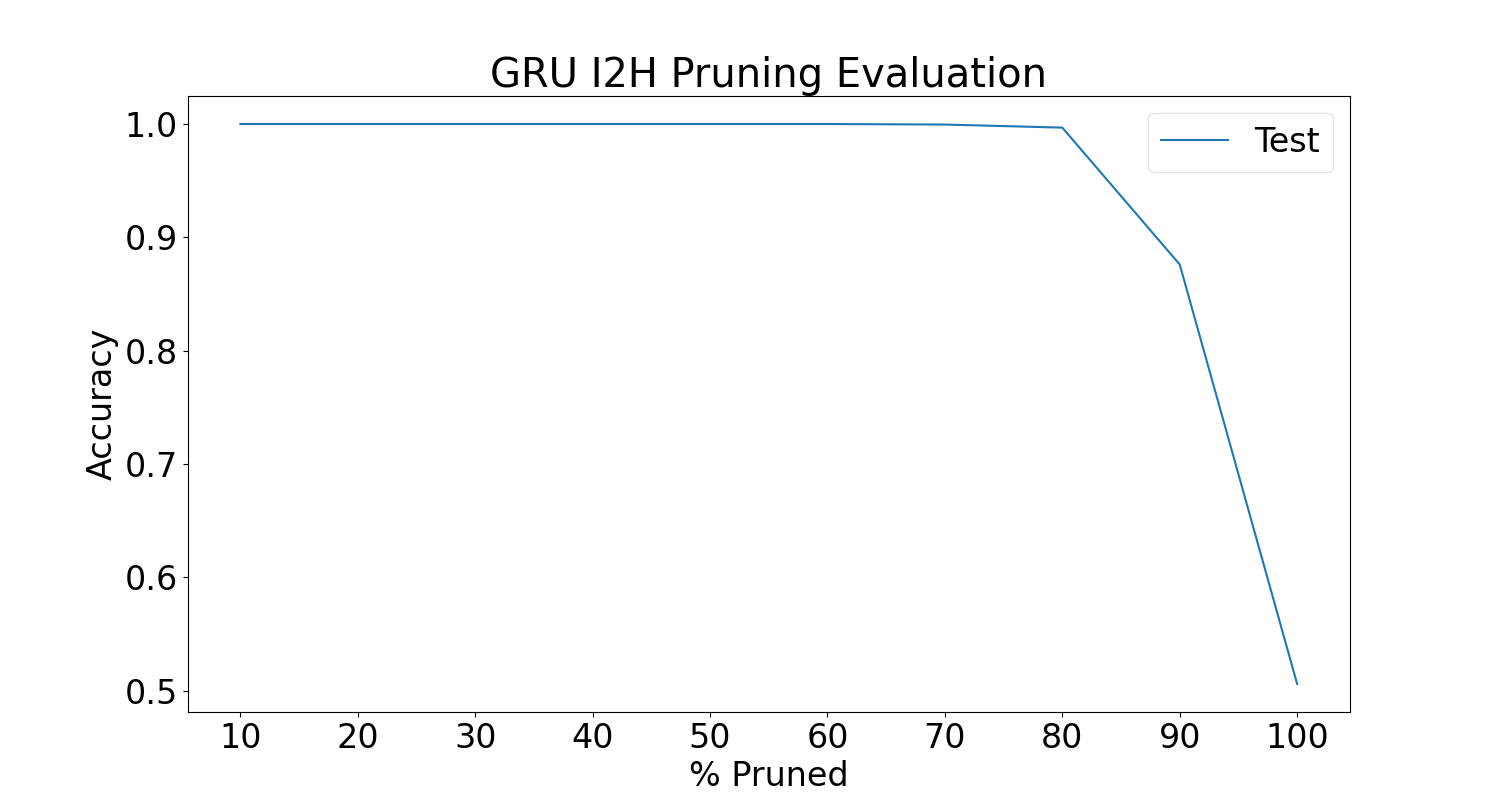
\includegraphics[width=0.8\linewidth]{images/results/pruning_i2h/gru_i2h_pruning_evaluation.png}
	\caption[GRU base model performance after pruning i2h weights]%
	{Base model performance of GRU after pruning only input-to-hidden weights. The pruning starts from $10\%$ and ends at $100\%$ with an increment of $10$ after each pruning round.}
	\label{fig:gru_i2h_prune}
\end{figure}

As we can see in the above graph, the model performs consistently at above 95\% accuracy with 80\% pruning. The model's performance drops sharply at 90\% pruning and returns baseline accuracy at 100\% pruning. Figure \ref{fig:gru_i2h_prune_regain} shows the number of epochs it takes for the GRU model to recover after pruning 90\%, and 100\% of its input-to-hidden weights.

\begin{figure}[h]
	\centering
	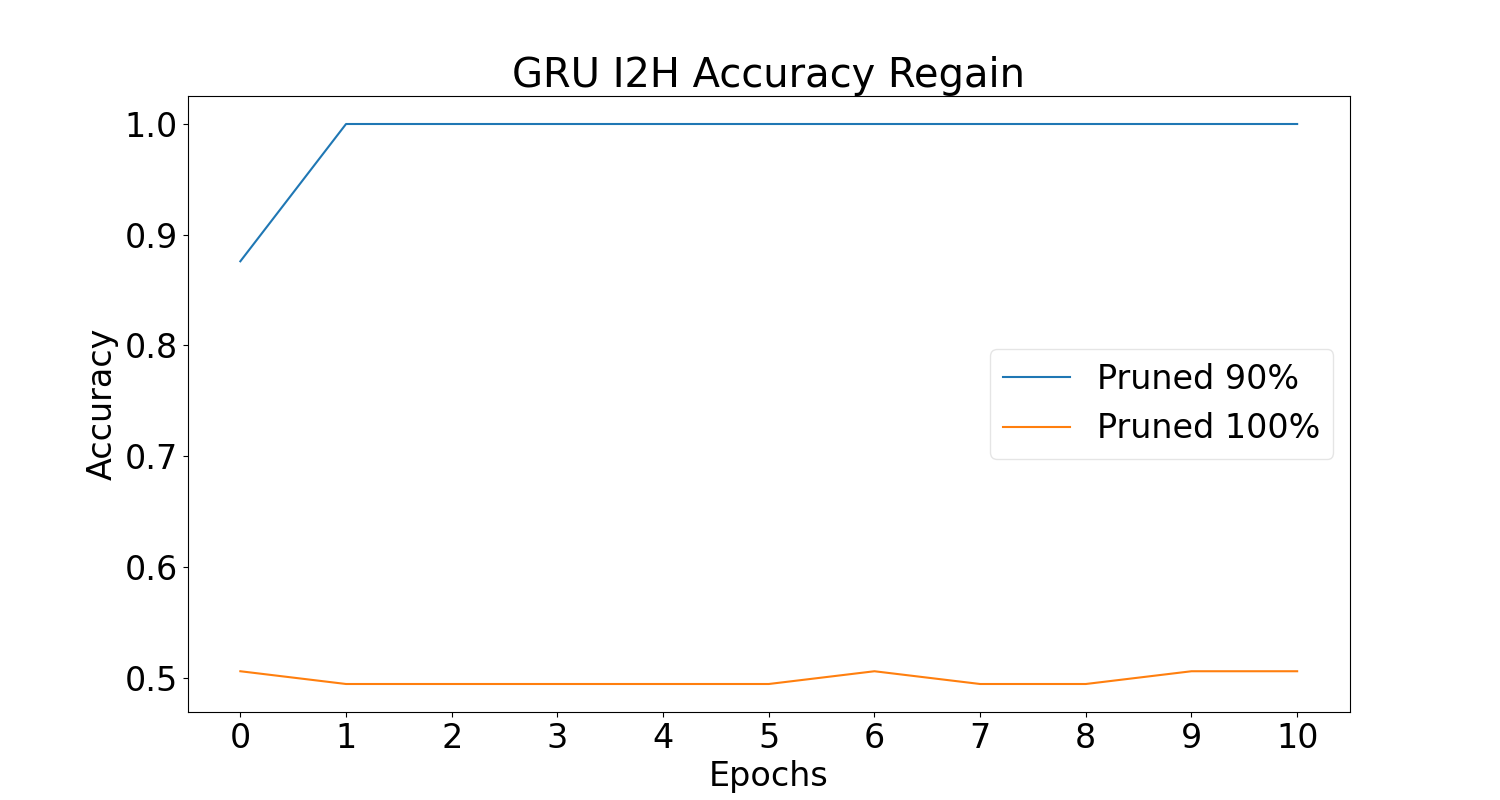
\includegraphics[width=0.8\linewidth]{images/results/pruning_i2h/gru_i2h_accuracy_regain.png}
	\caption[GRU base model performance regain after pruning i2h weights]%
	{The number of epochs required to regain the accuracy of GRU model after pruning 90\%, and 100\% of input-to-hidden weights.}
	\label{fig:gru_i2h_prune_regain}
\end{figure}

As we can see in the above graph, it only takes one epoch for the GRU model to recover from pruning 90\% of its input-to-hidden weights. The model never recovers from pruning 100\% of its input-to-hidden weights.

\subsection{Pruning only hidden-to-hidden weights}

In this section, we present the plots visualizing the effects of pruning only hidden-to-hidden weights on each RNN variant's performance.

Beginning with RNN with Tanh nonlinearity, as visualized in figure \ref{fig:rnn_tanh_h2h_prune}, the model performs consistently at above 90\% at 80\% of hidden-to-hidden weights pruned. We observe a sharp drop in accuracy at 90\% pruning, while the model returns baseline accuracy at 100\% pruning.

\begin{figure}[h]
	\centering
	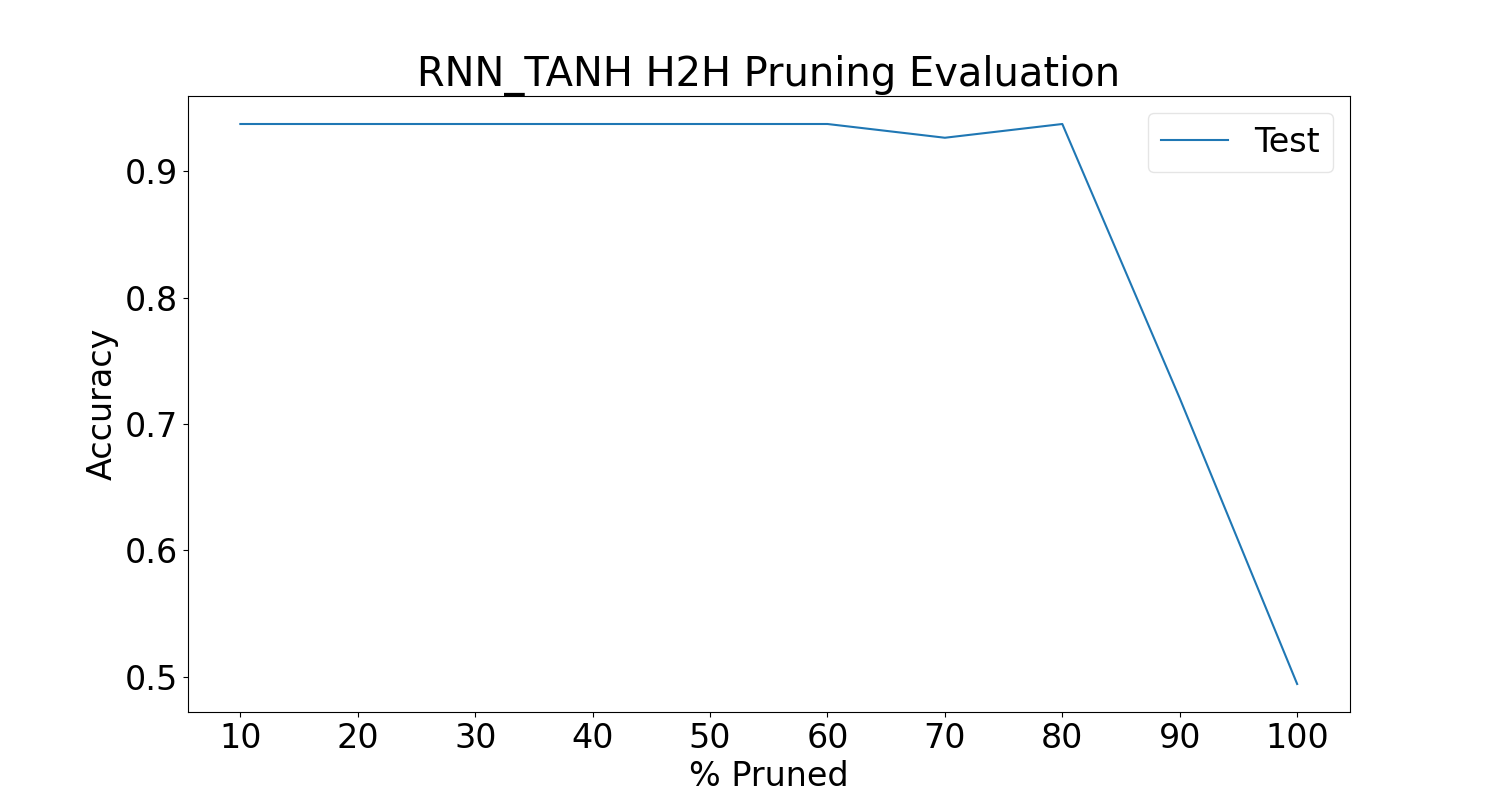
\includegraphics[width=0.8\linewidth]{images/results/pruning_h2h/rnn_tanh_h2h_pruning_evaluation.png}
	\caption[RNN\_Tanh base model performance after pruning h2h weights]%
	{Base model performance of RNN with Tanh nonlinearity after pruning only hidden-to-hidden weights. The pruning starts from $10\%$ and ends at $100\%$ with an increment of $10$ after each pruning round.}
	\label{fig:rnn_tanh_h2h_prune}
\end{figure}

Since performance drops only at 90\% and above of pruning, we perform an accuracy regain experiment for only 90\% and 100\% pruning of hidden-to-hidden weights as shown in figure \ref{fig:rnn_tanh_h2h_prune_regain}.

\begin{figure}[H]
	\centering
	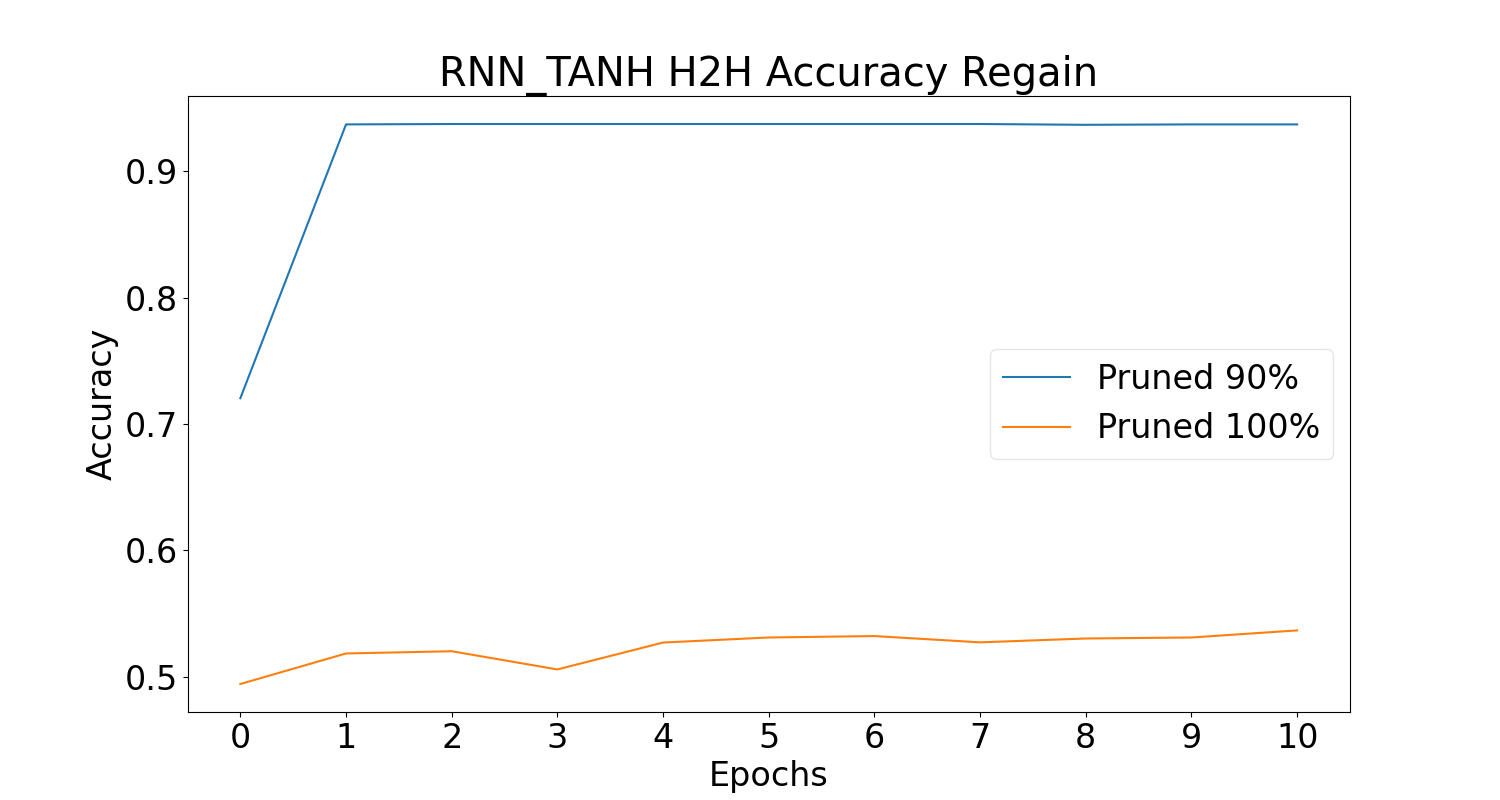
\includegraphics[width=0.8\linewidth]{images/results/pruning_h2h/rnn_tanh_h2h_accuracy_regain.png}
	\caption[RNN\_Tanh base model performance regain after pruning h2h weights]%
	{The number of epochs required to regain the accuracy of RNN\_Tanh model after pruning 80\%, 90\%, and 100\% of hidden-to-hidden weights.}
	\label{fig:rnn_tanh_h2h_prune_regain}
\end{figure}

As shown in the above graph, it only takes one epoch for the model to recover from 90\% of hidden-to-hidden weights pruned, while the model never recovers after pruning 100\% of hidden-to-hidden weights.

Next, we look at the effect of pruning hidden-to-hidden weights on the performance of RNN with ReLU nonlinearity. As shown in the below figure, the model performs consistently at above 95\% accuracy at 70\% pruning and starts dropping the performance from 80\% of pruning.

\begin{figure}[h]
	\centering
	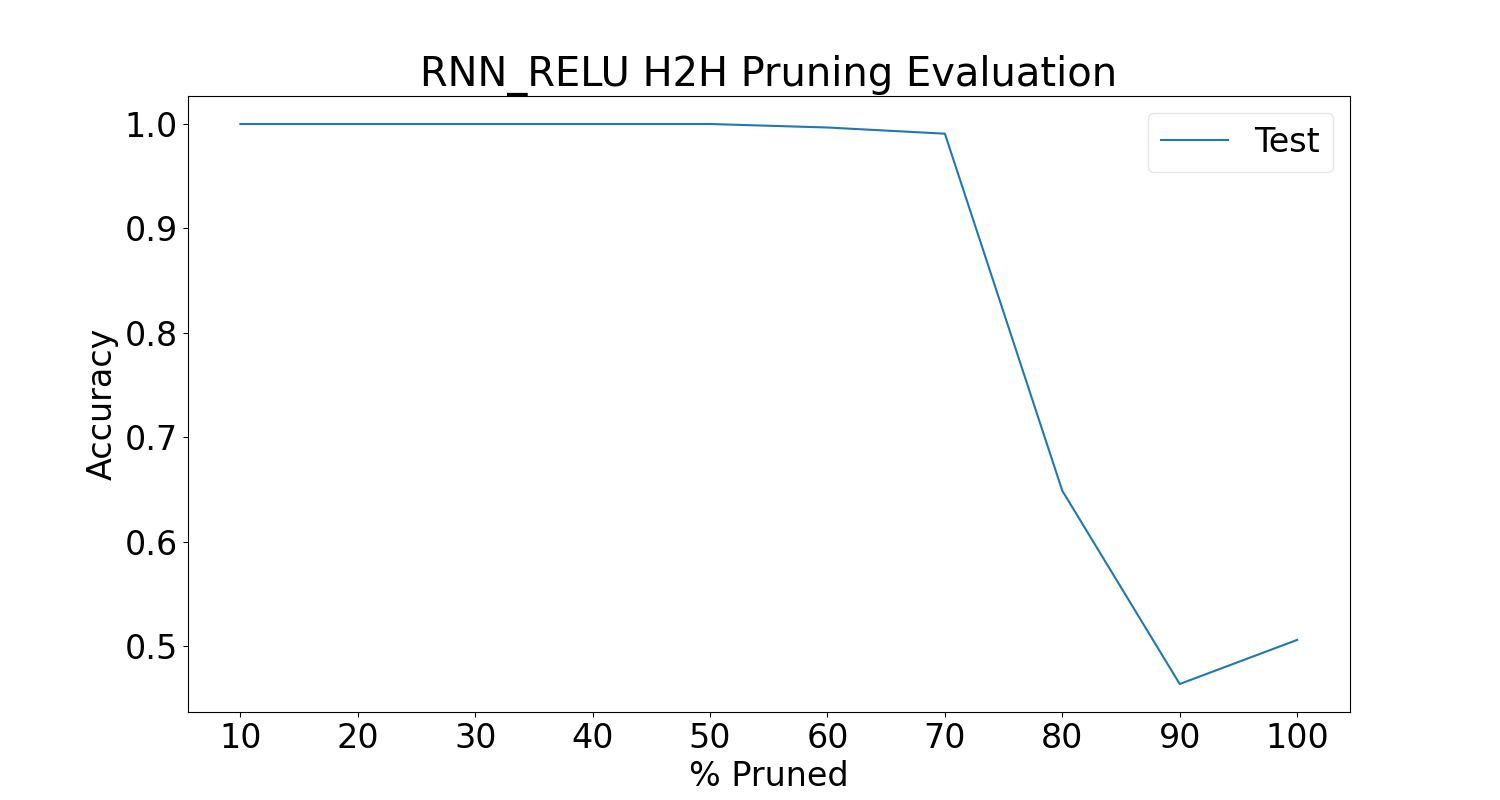
\includegraphics[width=0.8\linewidth]{images/results/pruning_h2h/rnn_relu_h2h_pruning_evaluation.png}
	\caption[RNN\_ReLU base model performance after pruning h2h weights]%
	{Base model performance of RNN with ReLU nonlinearity after pruning only hidden-to-hidden weights. The pruning starts from $10\%$ and ends at $100\%$ with an increment of $10$ after each pruning round.}
	\label{fig:rnn_relu_h2h_prune}
\end{figure}

The following graph shows the required number of epochs for the RNN with ReLU nonlinearity to recover from 80\%, 90\%, and 100\% pruning.

\begin{figure}[H]
	\centering
	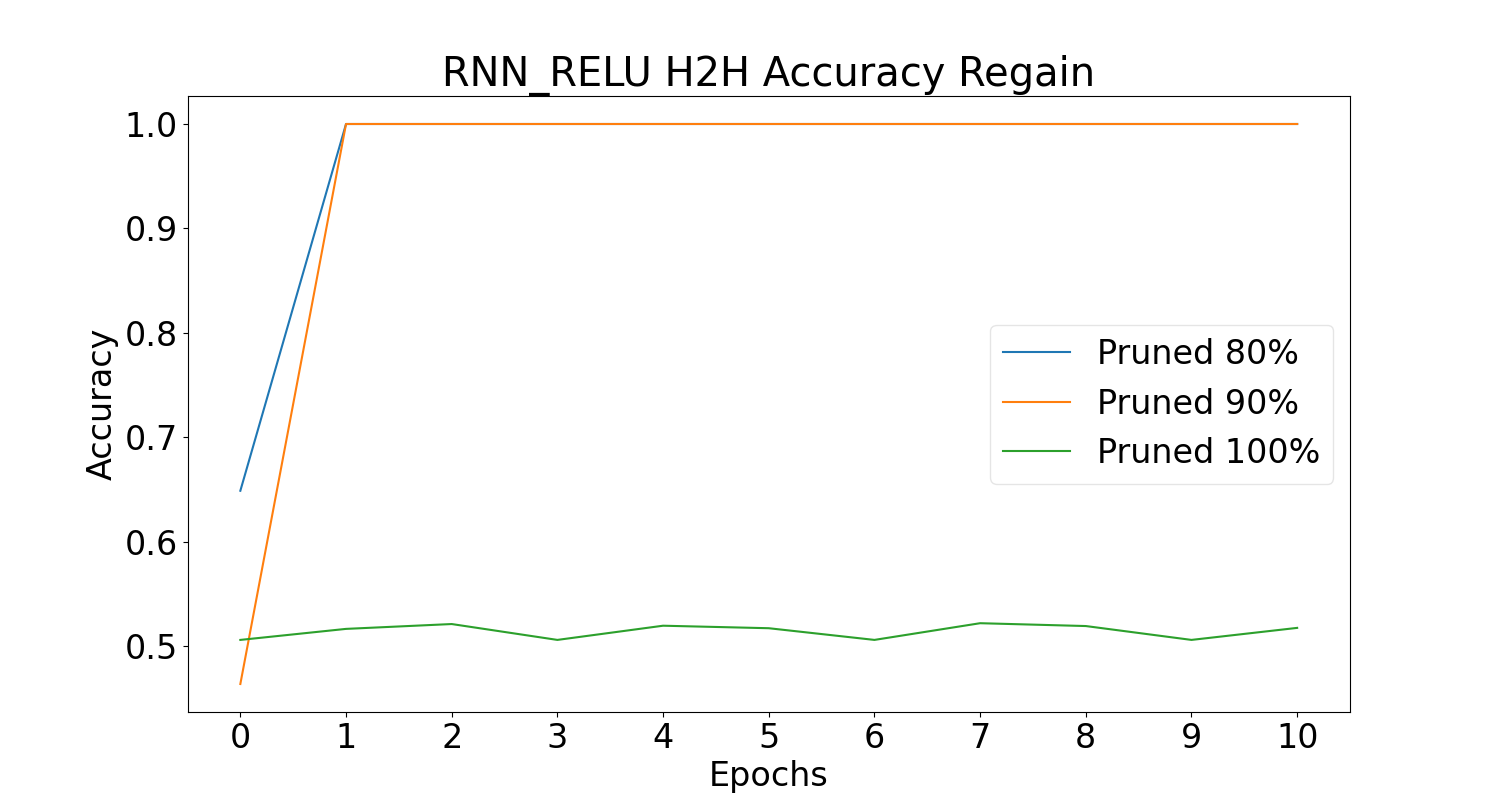
\includegraphics[width=0.8\linewidth]{images/results/pruning_h2h/rnn_relu_h2h_accuracy_regain.png}
	\caption[RNN\_ReLU base model performance regain after pruning h2h weights]%
	{The number of epochs required to regain the accuracy of RNN\_ReLU model after pruning 80\%, 90\%, and 100\% of hidden-to-hidden weights.}
	\label{fig:rnn_relu_h2h_prune_regain}
\end{figure}

As shown in the above figure, the model only requires one epoch to recover from 80\% and 90\% of hidden-to-hidden weights pruning. The model, as before, never recovers from 100\% pruning.

Next, we look at the effect of pruning hidden-to-hidden weights on the performance of LSTM, where, as shown in figure \ref{fig:lstm_h2h_prune}, the model performs consistently at around 95\% accuracy at 90\% pruning and drops the performance at 100\% of pruning.

\begin{figure}[h]
	\centering
	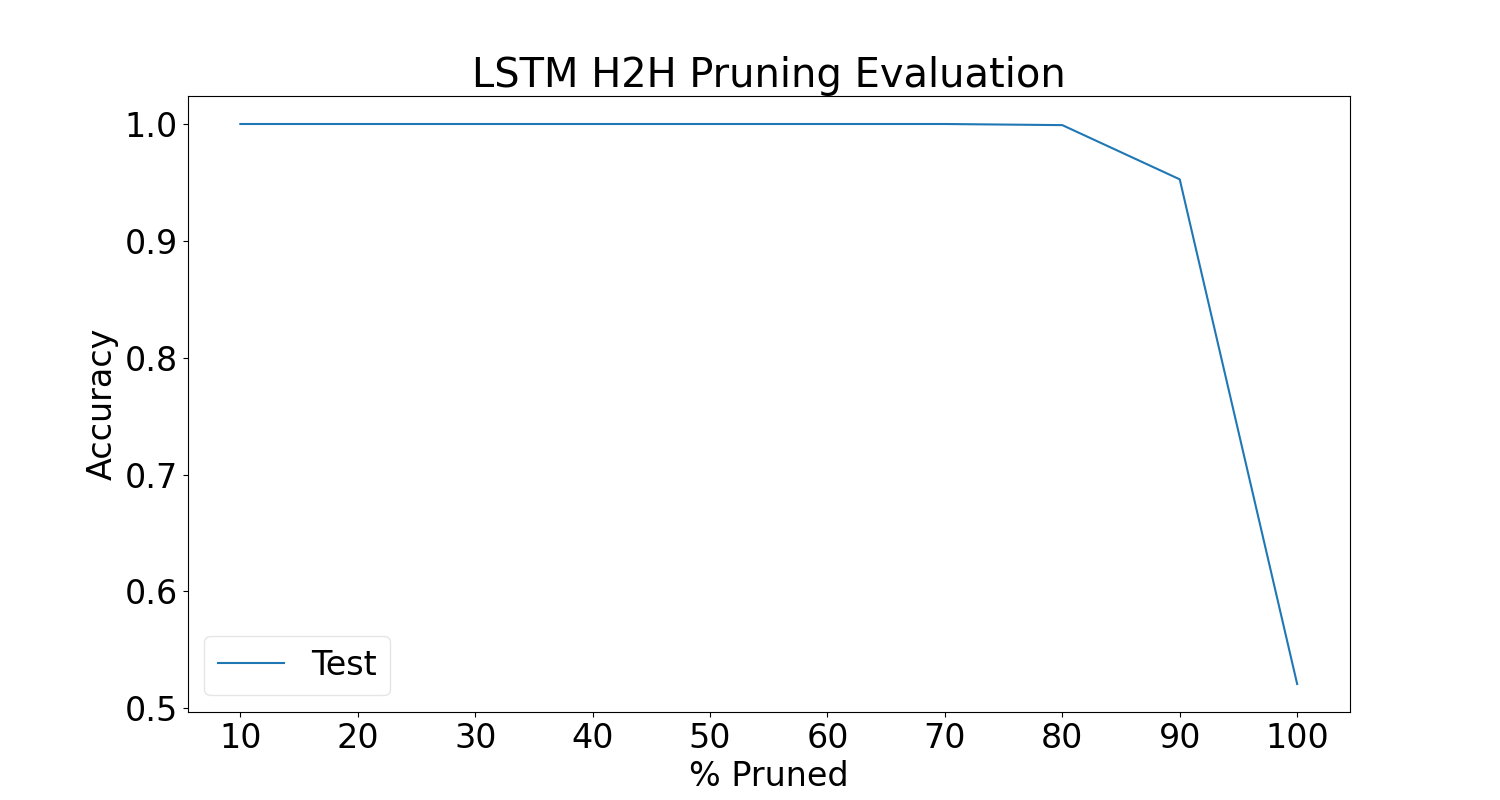
\includegraphics[width=0.8\linewidth]{images/results/pruning_h2h/lstm_h2h_pruning_evaluation.png}
	\caption[LSTM base model performance after pruning h2h weights]%
	{Base model performance of LSTM after pruning only hidden-to-hidden weights. The pruning starts from $10\%$ and ends at $100\%$ with an increment of $10$ after each pruning round.}
	\label{fig:lstm_h2h_prune}
\end{figure}

The following graph shows the required number of epochs for the LSTM to recover from 100\% pruning.

\begin{figure}[h]
	\centering
	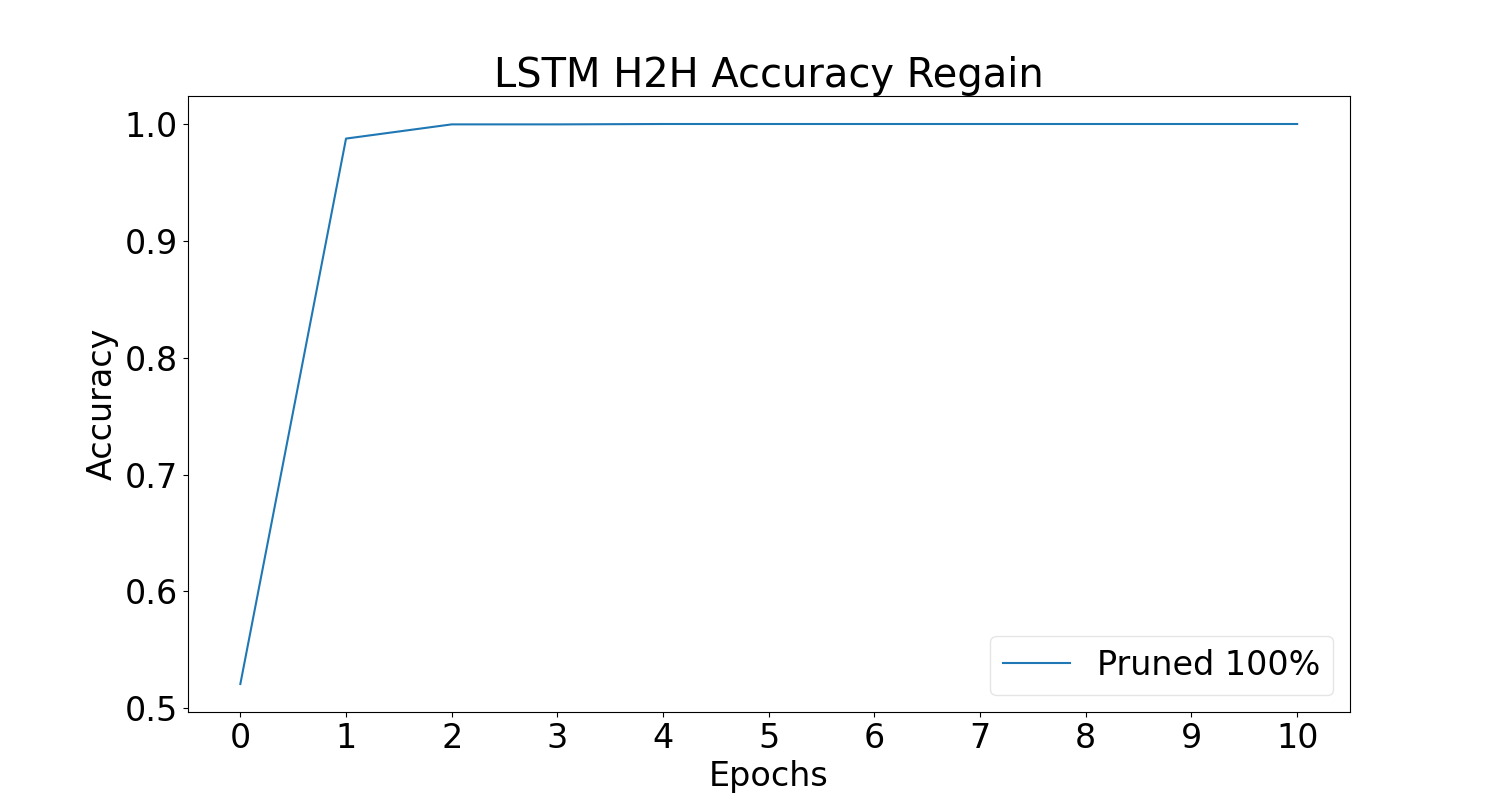
\includegraphics[width=0.8\linewidth]{images/results/pruning_h2h/lstm_h2h_accuracy_regain.png}
	\caption[LSTM base model performance regain after pruning h2h weights]%
	{The number of epochs required to regain the accuracy of LSTM model after pruning 100\% of hidden-to-hidden weights.}
	\label{fig:lstm_h2h_prune_regain}
\end{figure}

As shown in the above figure, even at 100\% pruning of hidden-to-hidden weights, the model still recovers in just one epoch. The reason behind this recovery is the existence of a cell state, as explained in section \ref{section:lstm}.

Finally, similar to LSTM, GRU also performs consistently at around 95\% at 90\% of hidden-to-hidden weights pruning, as shown in the following figure:

\begin{figure}[h]
	\centering
	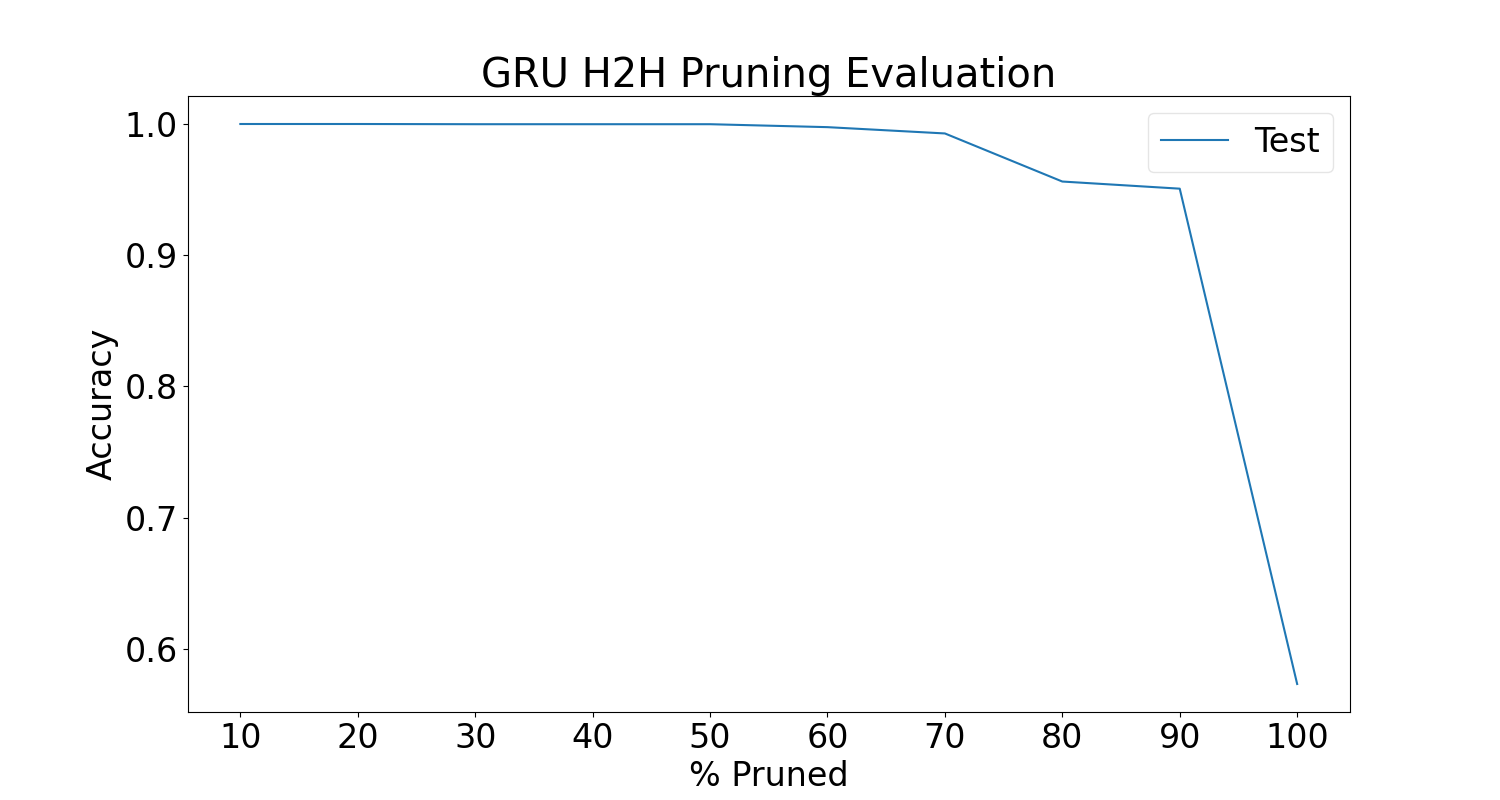
\includegraphics[width=0.8\linewidth]{images/results/pruning_h2h/gru_h2h_pruning_evaluation.png}
	\caption[GRU base model performance after pruning h2h weights]%
	{Base model performance of GRU after pruning only hidden-to-hidden weights. The pruning starts from $10\%$ and ends at $100\%$ with an increment of $10$ after each pruning round.}
	\label{fig:gru_h2h_prune}
\end{figure}

The following graph shows the required number of epochs for the GRU to recover from 100\% pruning.

\begin{figure}[h]
	\centering
	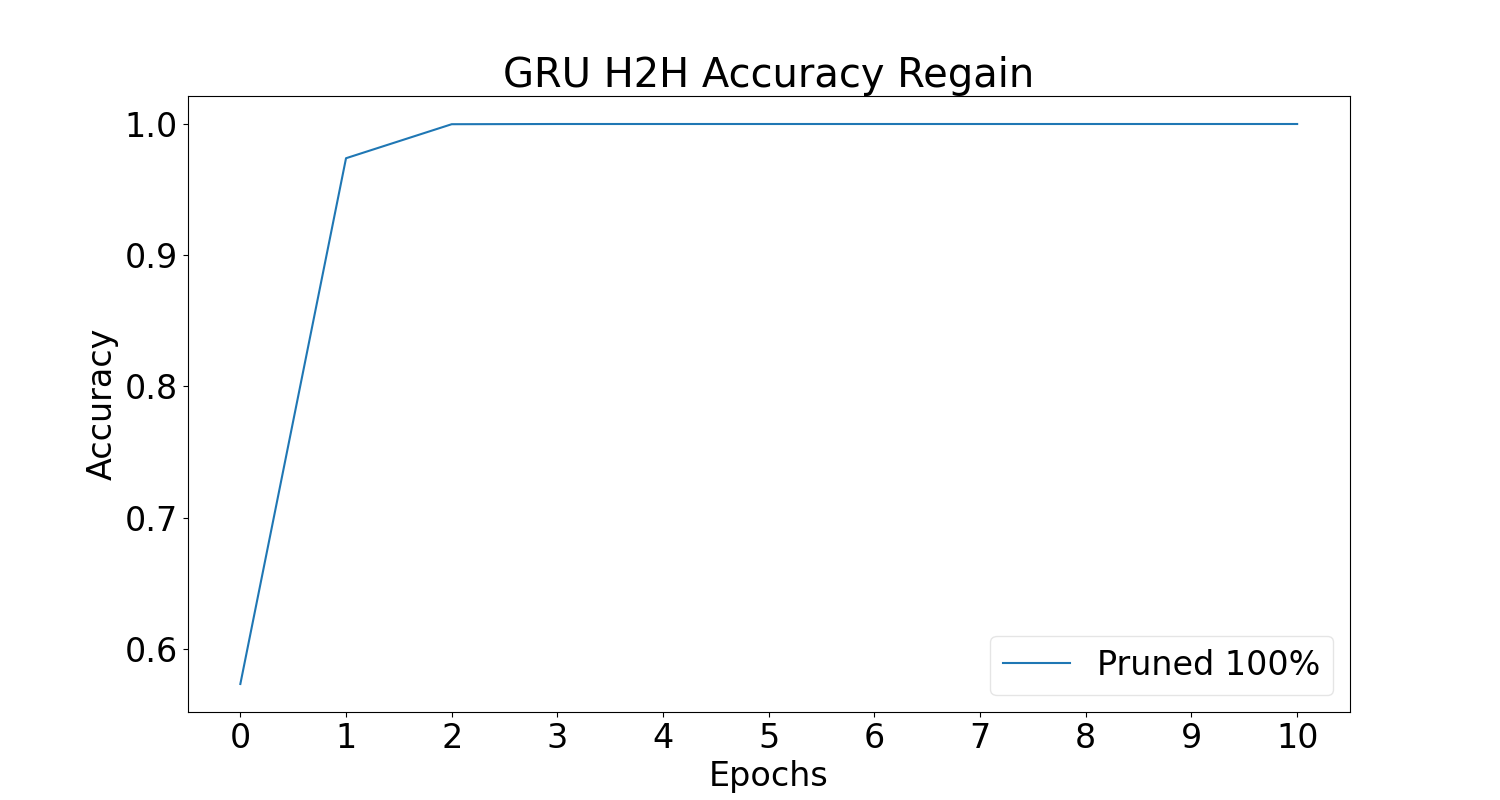
\includegraphics[width=0.8\linewidth]{images/results/pruning_h2h/gru_h2h_accuracy_regain.png}
	\caption[GRU base model performance regain after pruning h2h weights]%
	{The number of epochs required to regain the accuracy of GRU model after pruning 100\% of hidden-to-hidden weights.}
	\label{fig:gru_h2h_prune_regain}
\end{figure}

Like the LSTM model, even at 100\% pruning of hidden-to-hidden weights, the model still recovers in just one epoch, and after two epochs, the model returns 100\% accuracy.

This concludes the results of the pruning experiment. In the next section, we present the results of our randomly structured recurrent networks.

% -----------------------------------------------------------------------------------------------------------
% ------------------------------------------------ R. ST. RN ------------------------------------------------
% -----------------------------------------------------------------------------------------------------------

\section{Performance of Randomly Structured Recurrent Networks}\label{section:r_st_rn}

Our second experiment was to construct a random structure recurrent network using a random graph and train it on the Reber grammar dataset. During this training, we record different graph properties of the base random graph and try to correlate it with the test performance. In this section, we present the results of this experiment.

\subsection{Randomly Structured RNN with Tanh nonlinearity}

We begin with the plot that compares the accuracy of the Watts–Strogatz model and Barabási–Albert model based random structure RNN\_Tanh.

\begin{figure}[h]
	\centering
	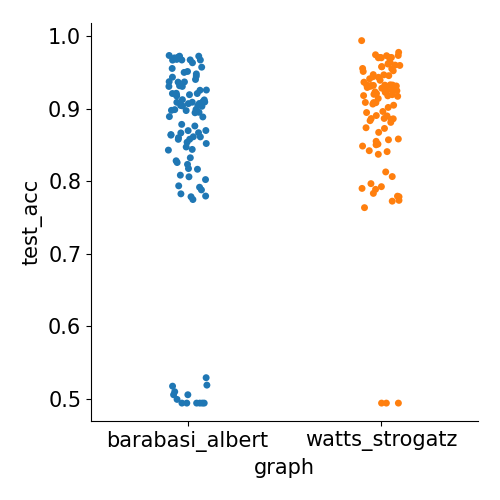
\includegraphics[width=0.45\linewidth]{images/results/random/tanh/graph_test_acc.png}
	\caption[Performance of the WS and BA based random structure RNN\_Tanh]%
	{Plot comparing the performance of the Watts–Strogatz and Barabási–Albert model based random structure RNN\_Tanh.}
	\label{fig:tanh_acc_comp}
\end{figure}

Next, the following table shows the Pearson correlation between test accuracy and different graph and recurrent network properties. The corresponding important plots are later shown in appendix \ref{app:rs_tanh}.

\begin{table}[h]
	\centering
	\begin{tabular}{|l|c|}
	    \hline
		\textbf{Property} & \textbf{Correlation with $test\_acc$}\\
		\hline
		layers & 0.25\\
		nodes & \textbf{0.40}\\
		edges & 0.38\\
		source\_nodes & 0.35\\
		diameter & -0.23\\
		density & 0.29\\
		average\_shortest\_path\_length & -0.27\\
		eccentricity\_var & -0.22\\
		degree\_var & -0.28\\
		closeness\_var & \textbf{-0.46}\\
		nodes\_betweenness\_var & \textbf{-0.49}\\
		edge\_betweenness\_var & -0.34\\
		\hline
	\end{tabular}
	\caption[Pearson correlation between test accuracy of RNN\_Tanh and different graph and recurrent network properties]{Pearson correlation between test accuracy of RNN\_Tanh and different graph and recurrent network properties}
	\label{tab:tanh_corr}
\end{table}

\subsection{Randomly Structured RNN with ReLU nonlinearity}

As with RNN\_Tanh, we begin with the plot that compares the accuracy of the Watts–Strogatz model and Barabási–Albert model based random structure RNN\_ReLU.

\begin{figure}[H]
	\centering
	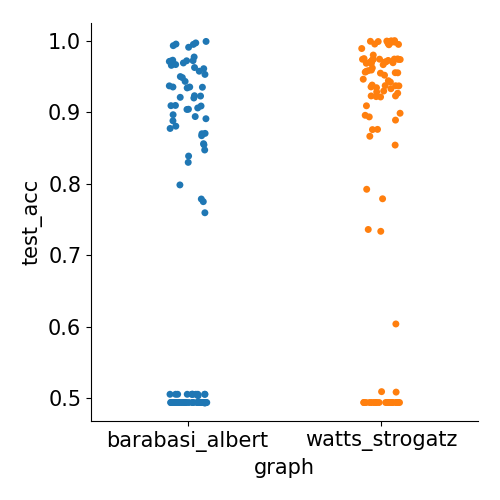
\includegraphics[width=0.45\linewidth]{images/results/random/relu/graph_test_acc.png}
	\caption[Performance of the WS and BA based random structure RNN\_ReLU]%
	{Plot comparing the performance of the Watts–Strogatz and Barabási–Albert model based random structure RNN\_ReLU.}
	\label{fig:relu_acc_comp}
\end{figure}

Next, the following table shows the Pearson correlation between test accuracy and different graph and recurrent network properties. The corresponding important plots are later shown in appendix \ref{app:rs_relu}.

\begin{table}[h]
	\centering
	\begin{tabular}{|l|c|}
	    \hline
		\textbf{Property} & \textbf{Correlation with $test\_acc$}\\
		\hline
		layers & 0.30\\
		nodes & \textbf{0.44}\\
		edges & \textbf{0.43}\\
		source\_nodes & \textbf{0.47}\\
		diameter & -0.27\\
		density & 0.15\\
		average\_shortest\_path\_length & -0.25\\
		eccentricity\_var & -0.24\\
		degree\_var & -0.26\\
		closeness\_var & -0.39\\
		nodes\_betweenness\_var & \textbf{-0.41}\\
		edge\_betweenness\_var & -0.30\\
		\hline
	\end{tabular}
	\caption[Pearson correlation between test accuracy of RNN\_ReLU and different graph and recurrent network properties]{Pearson correlation between test accuracy of RNN\_ReLU and different graph and recurrent network properties}
	\label{tab:relu_corr}
\end{table}

\subsection{Randomly Structured LSTM}

As before, we begin with the plot that compares the accuracy of the Watts–Strogatz model and Barabási–Albert model based random structure LSTM.

\begin{figure}[H]
	\centering
	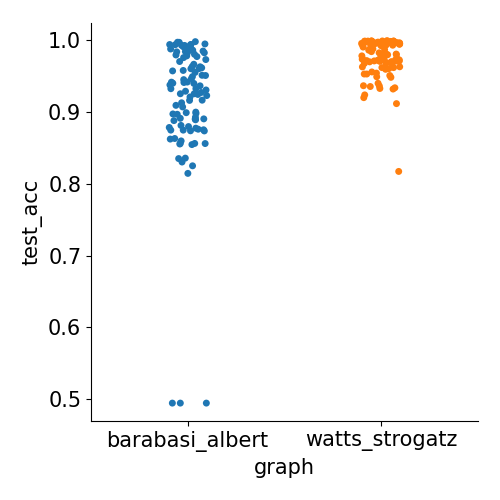
\includegraphics[width=0.45\linewidth]{images/results/random/lstm/graph_test_acc.png}
	\caption[Performance of the WS and BA based random structure LSTM]%
	{Plot comparing the performance of the Watts–Strogatz and Barabási–Albert model based random structure LSTM.}
	\label{fig:lstm_acc_comp}
\end{figure}

Next, the following table shows the Pearson correlation between test accuracy and different graph and recurrent network properties. The corresponding important plots are later shown in appendix \ref{app:rs_lstm}.

\begin{table}[h]
	\centering
	\begin{tabular}{|l|c|}
	    \hline
		\textbf{Property} & \textbf{Correlation with $test\_acc$}\\
		\hline
		layers & 0.28\\
		nodes & \textbf{0.44}\\
		edges & \textbf{0.42}\\
		source\_nodes & \textbf{0.57}\\
		diameter & -0.32\\
		density & 0.29\\
		average\_shortest\_path\_length & -0.36\\
		eccentricity\_var & -0.30\\
		degree\_var & -0.39\\
		closeness\_var & \textbf{-0.51}\\
		nodes\_betweenness\_var & \textbf{-0.56}\\
		edge\_betweenness\_var & \textbf{-0.44}\\
		\hline
	\end{tabular}
	\caption[Pearson correlation between test accuracy of LSTM and different graph and recurrent network properties]{Pearson correlation between test accuracy of LSTM and different graph and recurrent network properties}
	\label{tab:lstm_corr}
\end{table}

\subsection{Randomly Structured GRU}

As with LSTM, we begin with the plot that compares the accuracy of the Watts–Strogatz model and Barabási–Albert model based random structure GRU.

\begin{figure}[H]
	\centering
	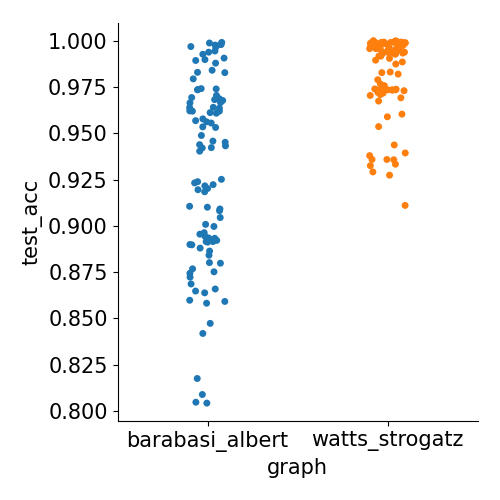
\includegraphics[width=0.45\linewidth]{images/results/random/gru/graph_test_acc.png}
	\caption[Performance of the WS and BA based random structure GRU]%
	{Plot comparing the performance of the Watts–Strogatz and Barabási–Albert model based random structure GRU.}
	\label{fig:gru_acc_comp}
\end{figure}

Next, the following table shows the Pearson correlation between test accuracy and different graph and recurrent network properties. The corresponding important plots are later shown in appendix \ref{app:rs_gru}.

\begin{table}[h]
	\centering
	\begin{tabular}{|l|c|}
	    \hline
		\textbf{Property} & \textbf{Correlation with $test\_acc$}\\
		\hline
		layers & 0.34\\
		nodes & \textbf{0.49}\\
		edges & \textbf{0.49}\\
		source\_nodes & \textbf{0.74}\\
		diameter & -0.20\\
		density & 0.34\\
		average\_shortest\_path\_length & -0.23\\
		eccentricity\_var & -0.21\\
		degree\_var & \textbf{-0.58}\\
		closeness\_var & \textbf{-0.67}\\
		nodes\_betweenness\_var & \textbf{-0.52}\\
		edge\_betweenness\_var & -0.26\\
		\hline
	\end{tabular}
	\caption[Pearson correlation between test accuracy of GRU and different graph and recurrent network properties]{Pearson correlation between test accuracy of GRU and different graph and recurrent network properties}
	\label{tab:gru_corr}
\end{table}

Positive Pearson correlation values in tables \ref{tab:tanh_corr}, \ref{tab:relu_corr}, \ref{tab:lstm_corr}, and \ref{tab:gru_corr} indicate that an increase in the property variable increases test accuracy. Similarly, a negative Pearson correlation in the same tables indicates that a decrease in the property variable decreases the test accuracy. A higher positive or negative correlation indicates a strong relationship between a graph property and test corresponding test accuracy.

\section{Performance prediction}

While training randomly structured recurrent networks, we create a small dataset by storing all the graph and recurrent network properties and their corresponding test accuracy. We train three regressor algorithms on this dataset, and based on the resulting R-squared value, we determine if it is possible to predict a randomly structured recurrent network's performance.

For each RNN variant, the following table shows the R-squared values from each regressor algorithm we used:

\begin{table}[h]
	\centering
	\begin{tabular}{|c||c|c|c|}
	    \hline
		\textbf{RNN Variant} & \textbf{Bayesian Ridge} & \textbf{Random Forest} & \textbf{AdaBoost}\\
		\hline
		RNN\_Tanh & 0.47919 & 0.43163 & 0.35698\\
		RNN\_ReLU & 0.36075 & 0.61504 & 0.53469\\
		LSTM & 0.37206 & 0.57933 & 0.59514\\
		GRU & 0.67224 & 0.87635 & 0.78313\\
		\hline
	\end{tabular}
	\caption[R-squared values from each regressor algorithm, for each RNN variant]{R-squared values from each regressor algorithm for each RNN variant help determine our data's closeness to the fitted regression line. All four RNN variants presented in this table are randomly structured.}
	\label{tab:r-squared}
\end{table}

In simple words, the R-squared value helps us to understand how close our data is to the fitted regression line. A higher R-square value usually means that our data is a better fit for the model.

In our case, RNN\_Tanh has below 0.5 R-squared value for all three regressors, while RNN\_ReLU has a good R-squared value with Random Forest regressor (0.61). In contrast to RNN\_ReLU, LSTM has a better R-squared value with AdaBoost regressor, while GRU has excellent R-squared values for all three regressor algorithms.

Based on these results, we further experimented with Random Forest regressor and data from randomly structured RNN\_ReLU and randomly structured GRU to extract feature importance scores of different properties under different circumstances. Results from this experiment are shown in appendix \ref{app:tables}.